\documentclass[11pt]{article}
\usepackage[spanish]{babel}
\usepackage{translations}
\usepackage[titles]{tocloft}
\usepackage{multicol}
\usepackage{graphicx}
\usepackage{amsmath}
\usepackage{hyperref}
\usepackage{amsmath}
\usepackage{amssymb}
\usepackage{listings}
\usepackage{courier}
\usepackage[margin=1in]{geometry}
\usepackage{changepage}
\usepackage{titlesec}
\usepackage{wrapfig}
\usepackage[version=4]{mhchem}
\usepackage{multirow}
\usepackage{siunitx}
\usepackage{ragged2e}
\usepackage{adjustbox}
\usepackage[font=small,labelfont=bf]{caption}
\usepackage[table,xcdraw]{xcolor}
\usepackage{afterpage}
\usepackage{xfrac}
\usepackage{animate}
\usepackage{subcaption}

\definecolor{codegreen}{rgb}{0,0.6,0}
\definecolor{codegray}{rgb}{0.5,0.5,0.5}
\definecolor{codepurple}{rgb}{0.58,0,0.82}
\definecolor{backcolour}{rgb}{0.95,0.95,0.92}

\lstdefinestyle{mystyle}{
    backgroundcolor=\color{backcolour},   
    commentstyle=\color{codegreen},
    keywordstyle=\color{magenta},
    numberstyle=\tiny\color{codegray},
    stringstyle=\color{codepurple},
    basicstyle=\ttfamily\footnotesize,
    breakatwhitespace=false,         
    captionpos=b,                    
    keepspaces=true,                 
    numbers=left,                    
    numbersep=5pt,                  
    showspaces=false,                
    showstringspaces=false,
    showtabs=false,                  
    tabsize=2
}
\lstset{language=Python, 
        basicstyle=\ttfamily\small, 
        keywordstyle=\color{keywords},
        commentstyle=\color{comments},
        stringstyle=\color{red},
        showstringspaces=false,
        identifierstyle=\color{codepurple},
        keywords=[2]{pow},
        keywordstyle=[2]{\color{orange}},
}

\lstset{style=mystyle}
\setlength\parindent{0pt}
\renewcommand{\labelenumi}{\alph{enumi}.}

\setlength\parindent{0pt}

\renewcommand{\labelenumi}{\alph{enumi}.}
   
\newcommand{\titulo}{Trazado de Rayos \\\ \\(Práctica 1)}
\newcommand{\nombreestudiante}{Víctor Mira Ramírez\\ Rocío Ponsoda Orgilés}
\newcommand{\nombredirector}{María Inmaculada Pascual Villalobos}
\newcommand{\fecha}{\date{Noviembre 2023}}

\pagebreak

\renewcommand{\listtablename}{Índice de tablas} 
\renewcommand{\tablename}{Tabla} 
\renewcommand\cftsecdotsep{\cftdotsep}

\setlength{\cftbeforesecskip}{0.5ex}
\renewcommand{\cftsecfont}{%
  \fontsize{11}{13}\usefont{OT1}{phv}{bc}{n}\selectfont
}
\makeatletter
\renewcommand{\@pnumwidth}{1.75em}
\renewcommand{\@tocrmarg}{2.75em}
\makeatother

\begin{document}

\begin{titlepage}
	\centering
	
\includegraphics[width=65mm]{fotos/logoUA.png}\par
	\vspace{1cm}
	{\huge\bfseries \vspace{15mm} \titulo \par}
	\vfill
	{\large 
	\vfill
	Estudiantes:\par\vspace{2mm}
	\nombreestudiante\par
	\vfill
	Profesora:\par\vspace{2mm}
    \nombredirector
    \vfill
    Universidad de Alicante\par
    Facultad de Ciencias: Departamento de Óptica, Farmacología y Anatomía\par
    Óptica I\par
	\fecha\par}
\end{titlepage}

\pagebreak

\begin{abstract}\label{sec:abstract}
    %% ABSTRACT ORIGINAL %%
    % \noindent El objetivo de esta práctica es visualizar e interpretar el trazado de rayos paraxial y exacto a través de diferentes sistemas ópticos. Asimismo, se podrá observar la localización de los elementos cardinales de dichos sistemas y diferentes aberraciones ópticas.
    % Durante la primera sesión práctica se visualizarán conceptos teóricos mediante el manejo del programa. Durante la segunda parte de la práctica se simulará el trazado de rayos de diferentes instrumentos ópticos. Esta metodología permitirá la comprobación de los conocimientos adquiridos en teoría, así como su aplicación a la simulación de instrumentos ópticos reales.

    %% PROPUESTA DE ABSTRACT 1 %%
    % \noindent Los objetivos de esta práctica consisten en representar gráficamente e interpretar el trazado de rayos paraxiales y exactos a través de diversos sistemas ópticos. Además, se examinará la ubicación de los puntos cardinales en dichos sistemas, así como diversas aberraciones ópticas. A lo largo de la sesión práctica, se pusieron en práctica conceptos teóricos mediante la utilización del programa UB Optics. Esta metodología facilita la verificación de los conocimientos teóricos adquiridos y su aplicación en la simulación de instrumentos.

    %% PROPUESTA DE ABSTRACT 2 %%
    \noindent En esta práctica, nos sumergimos en la compleja tarea de visualizar y dar significado al trazado de rayos, ya sean paraxiales o exactos, a medida que atraviesan distintos sistemas ópticos. Al mismo tiempo, exploramos la disposición de los elementos cardinales en estos sistemas, así como diversas manifestaciones de aberraciones ópticas. Durante la sesión práctica, nos sumergimos en conceptos teóricos utilizando la plataforma UB Optics como medio conductor. Esta metodología no solo sirvió para confirmar los conocimientos teóricos adquiridos, sino también para aplicarlos de manera práctica en la simulación de instrumentos.
\end{abstract}

\vspace{0.3cm}
\tableofcontents
\newpage
\vspace{-0.2cm}


\section{Estudio de los parámetros y funcionamiento de las lentes}
    \subsection{Lentes Convergentes}
    \subsubsection{Cuestiones previas}
    \vspace{0.2cm}
    \begin{wrapfigure}[9]{r}{0.5\textwidth}
        \vspace{-0.6cm}
        \centering
        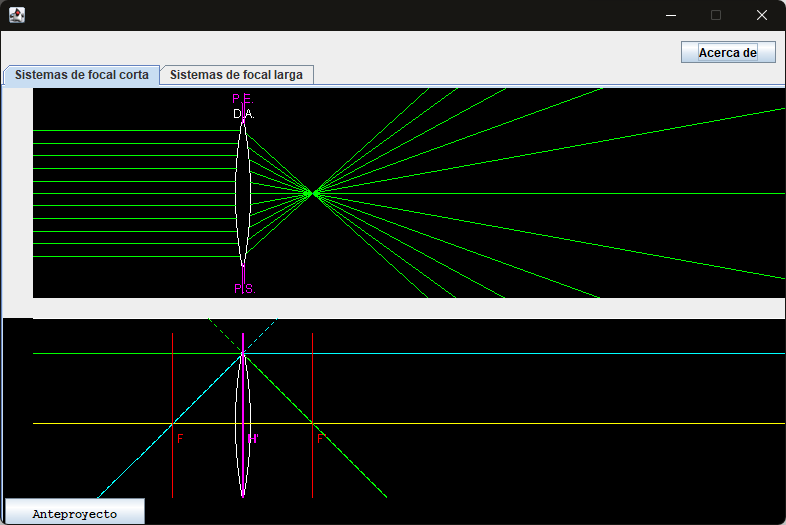
\includegraphics[width=0.49\textwidth]{fotos/parte 1/Lentes convergentes/previas_convergentes.png}
    \end{wrapfigure}
    
    \noindent Las cuestiones previas todas se realizaron alrededor de un sistema con las siguientes características:
    \begin{itemize}
        \item Lente de potencia $P = 20\ D$ en la posición $150.0\ mm$.
        \item Objeto real en infinito
    \end{itemize}
    Dicho sistema, junto con sus elementos cardinales, lo visualizamos en el programa \textit{UB Optics}.\\
    
    \vspace{5mm}
    \textit{CUESTIÓN 1.  ¿A qué distancia de la lente focalizan los rayos que provienen del punto objeto situado en infinito?}\\
    
    \noindent Tal y como hemos visto en la teoría de la asignatura, cuando un objeto está situado en infinito, los rayos que de él provienen convergen a una distancia de la lente equivalente a su distancia focal imagen.
    \begin{equation*}
        s' = f' = \frac{1}{P} = 50\ mm
    \end{equation*}
    \vspace{10mm}
    
    \textit{CUESTIÓN 2. Visualizar la pupila de entrada, la pupila de salida y el diafragma de apertura del sistema óptico. Pinchar en la pestaña elementos cardinales y comprobar dónde está situado el plano focal objeto y el plano focal imagen del sistema, así como sus planos principales.}\\
    
    \noindent En la parte inferior de la figura vienen representados los elementos cardinales del sistema. Podemos comprobar que tanto diafragma de apertura (DA) como pupila de entrada y de salida (PE y PS, respectivamente), corresponden a la lente, puesto que no tenemos ningún otro elemento que pueda desempeñar estas funciones. En cuanto a los planos principales H y H', también se encuentran en la lente.\\

    \clearpage
    \textit{CUESTIÓN 3.  Colocar ahora el objeto en la posición 50.0 mm, manteniendo la potencia de la lente. ¿A qué distancia de la lente focalizan los rayos que provienen del punto objeto? Visualizar los elementos cardinales del sistema.}\\
    
    \noindent En este caso tenemos el objeto situado sobre la distancia focal objeto. Esto implica, tanto por lo visto en teoría como por lo que vemos en la imagen, que los rayos convergerán a dos veces la distancia focal, es decir, $s' = 2f' = 100\ mm$. En la siguiente figura se representan los elementos cardinales:
    \begin{figure}[ht]
        \centering
        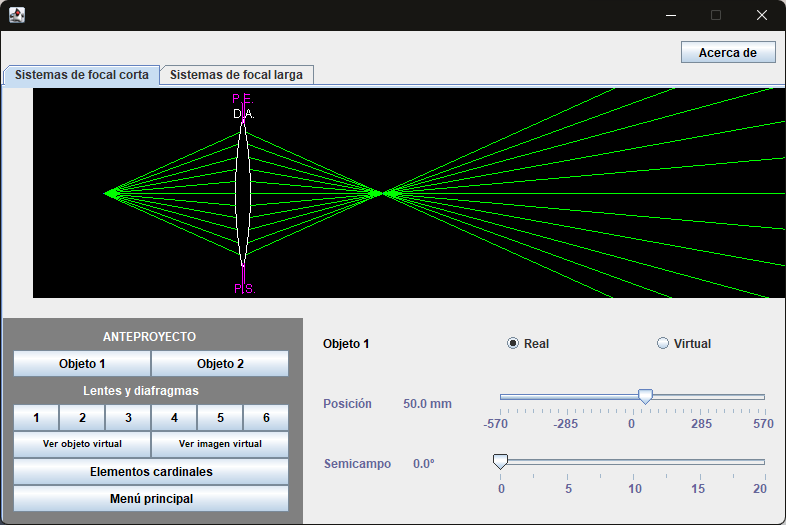
\includegraphics[width=0.49\textwidth]{fotos/parte 1/Lentes convergentes/previas_convergentes_1.png}
    \end{figure}
    \vspace{10mm}

    \textit{CUESTIÓN 4. Colocar un diafragma en la posición donde se forma la imagen del Objeto 1 del apartado anterior. Hacer clic en el número 2 para añadir un segundo elemento al sistema. Seleccionar el diámetro más pequeño posible de diafragma sin limitar la cantidad de luz que sale del objeto y llega a la imagen.}\\
    
    \noindent El sistema pedido es el que representamos.
    \begin{figure}[ht]
        \centering
        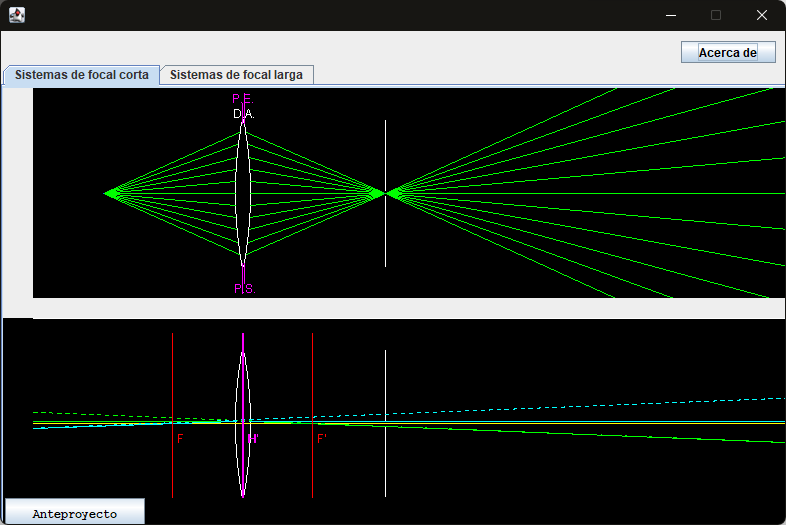
\includegraphics[width=0.49\textwidth]{fotos/parte 1/Lentes convergentes/previas_convergentes_3.png}
    \end{figure}

    
    \clearpage
    \textit{CUESTIÓN 5. Ahora desplazar la posición del objeto (Objeto 1) hasta situarlo en F, manteniendo la potencia de la lente y el tamaño del diafragma. ¿Quién actúa en este caso como diafragma de apertura del sistema, pupila de entrada y pupila de salida?}
    \vspace{0.3cm}
    
    \begin{wrapfigure}[10]{l}{0.5\textwidth}
        \vspace{-0.6cm}
        \centering
        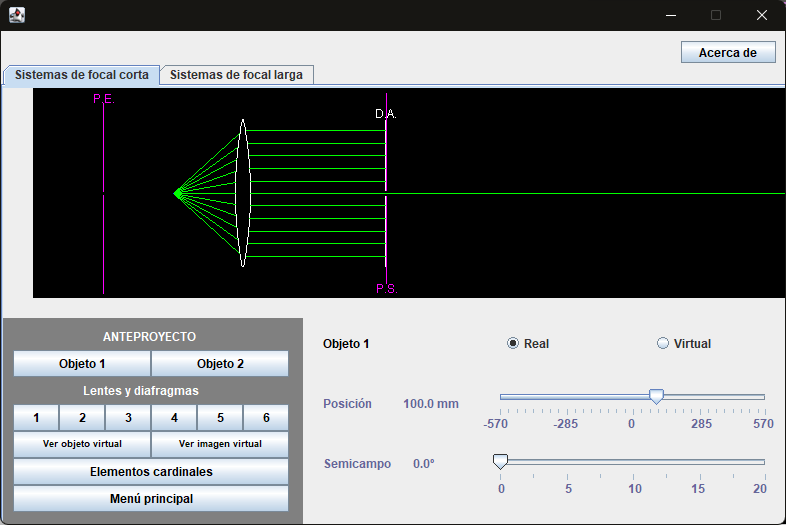
\includegraphics[width=0.49\textwidth]{fotos/parte 1/Lentes convergentes/previas_convergentes_4.png}
    \end{wrapfigure}
    
    \noindent La imagen en este caso se formará en el infinito, puesto que el objeto lo tenemos sobre el foco.\\
    
    Ahora los rayos sí se ven limitados por el diafragma y por tanto es diafragma de apertura (y también pupila de salida, ya que se encuentra en el espacio imagen). La pupila de entrada corresponde a la preimagen del diafragma a través de la lente.
    
    \vspace{20mm}
    \textit{CUESTIÓN 6. Mover el diafragma a la derecha y abrirlo al máximo. Mover la lente hasta la posición $250.0\ mm$. Colocar el objeto alejado, pero no en infinito. Selecciona un objeto fuera de eje, por ejemplo, un semicampo de 3.5 grados para ver el tamaño y orientación de la imagen formada a través de la lente.}\\
    
    \noindent El sistema planteado sobre el cual vamos a realizar cambios es el siguiente:
    \begin{figure}[ht]
        \centering
        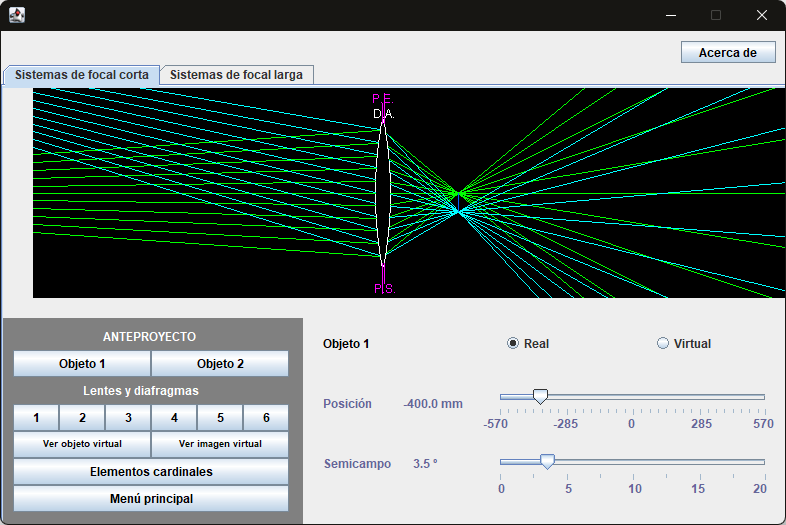
\includegraphics[scale= 0.4]{fotos/parte 1/Lentes convergentes/previas_convergentes_5.png}
    \end{figure}\\

    \clearpage
    \textit{Colocar el objeto un poco antes del punto F y comprobar las características de la imagen.}
    \begin{wrapfigure}[12]{r}{0.5\textwidth}
        \centering
        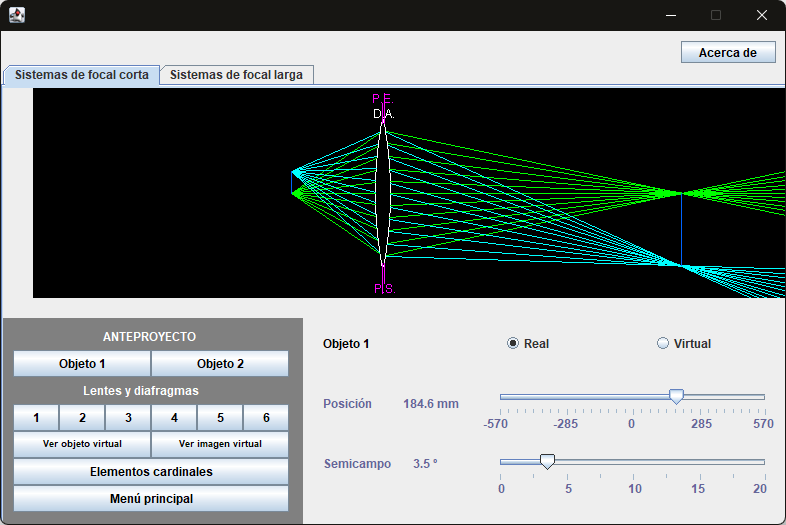
\includegraphics[width=0.49\textwidth]{fotos/parte 1/Lentes convergentes/previas_convergentes_6.png}
    \end{wrapfigure}

    \hspace{0cm}\\\hspace{0cm}\\\hspace{0cm}\\\hspace{0cm}\\\noindent En este caso podemos comprobar que la imagen queda de tamaño mucho mayor al tamaño original del objeto y que además es invertida.
    \\\hspace{0cm}\\\hspace{0cm}\\\hspace{0cm}\\\hspace{0cm}\\\hspace{0cm}\\
    
    \textit{Cambiar la posición del objeto a una distancia menor que la distancia focal objeto, volver a comprobar las características de la imagen. Apretar la opción ver imagen virtual.}

    \begin{wrapfigure}[9]{l}{0.5\textwidth}
        \centering
        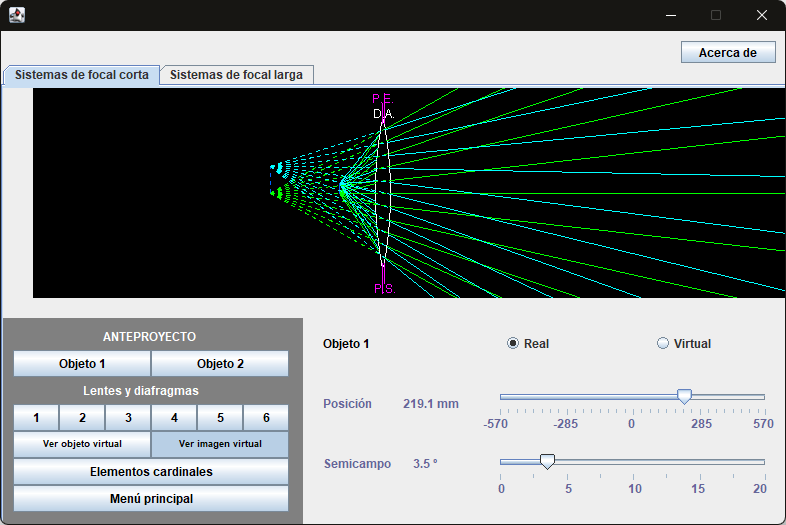
\includegraphics[width=0.49\textwidth]{fotos/parte 1/Lentes convergentes/previas_convergentes_7.png}
    \end{wrapfigure}\hspace{0cm}\\

    \hspace{0cm}\\\hspace{0cm}\\\noindent Ahora tenemos una imagen virtual (ya que se genera a partir de las prolongaciones de los rayos) a la izquierda de la lente. En cuanto a sus dimensiones, vemos que es mayor que el objeto y además no está invertida.\hspace{0cm}\\\hspace{0cm}\\\hspace{0cm}\\\hspace{0cm}\\\hspace{0cm}\\       

    \textit{Trabajar de nuevo con un semicampo de 0 grados y seleccionar el botón objeto 1 para cambiar a objeto virtual (activar el botón “ver objeto virtual”), desplazar la posición del objeto para ver cómo se forma la imagen.}\\

    \begin{wrapfigure}[11]{r}{0.5\textwidth}
        \vspace{-0.75cm}
        \centering
        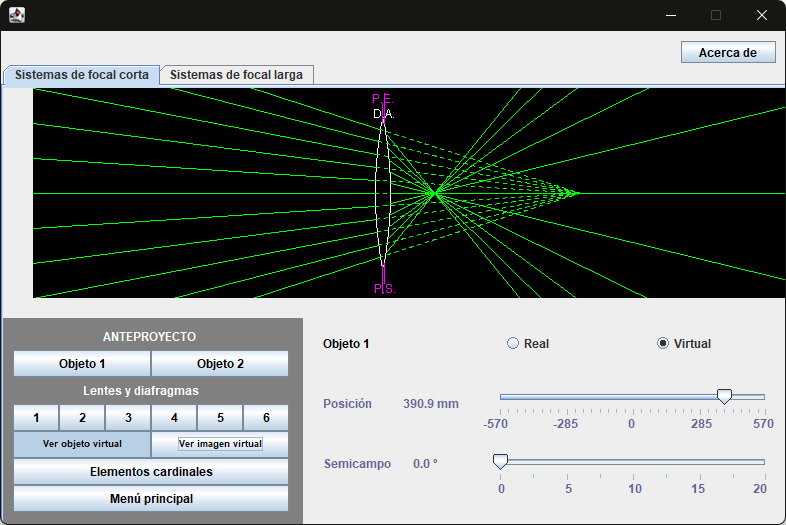
\includegraphics[width=0.49\textwidth]{fotos/parte 1/Lentes convergentes/propuesta_convergetnes_8.png}
    \end{wrapfigure}
    \hspace{0cm}\\\hspace{0cm}\\\hspace{0cm}\\
    Hemos elegido un objeto virtual situado a la derecha de la lente de forma que la imagen, que es real, se forma a la derecha de la lente (en el espacio entre esta y el objeto).
    
    \clearpage
    \subsubsection{Cuestiones propuestas}
    \textit{\textbf{CUESTIÓN 1.} Comprobar con una lente convergente y objeto en infinito (semicampo 3.5 grados) que el tamaño de la imagen aumenta al aumentar la distancia focal de la lente. Representarlo para tres focales distintas.}
    \\
    
    \noindent
    A continuación mostramos tres trazados de rayos para un mismo objeto en infinito y con semicampo $3.5^\circ$. Las tres lentes convergentes que se muestran están en la misma posición - tal y como se ve en la captura de pantalla - pero hemos variado su potencia y por lo tanto su distancia focal.\\
    
    \begin{figure}[ht]
        \centering
        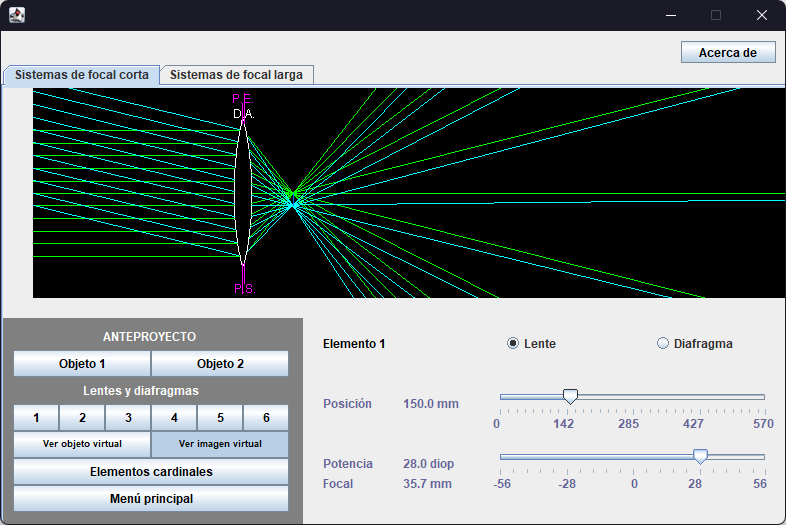
\includegraphics[width=0.49\textwidth]{fotos/parte 1/Lentes convergentes/convergentes_1_P28.png}
        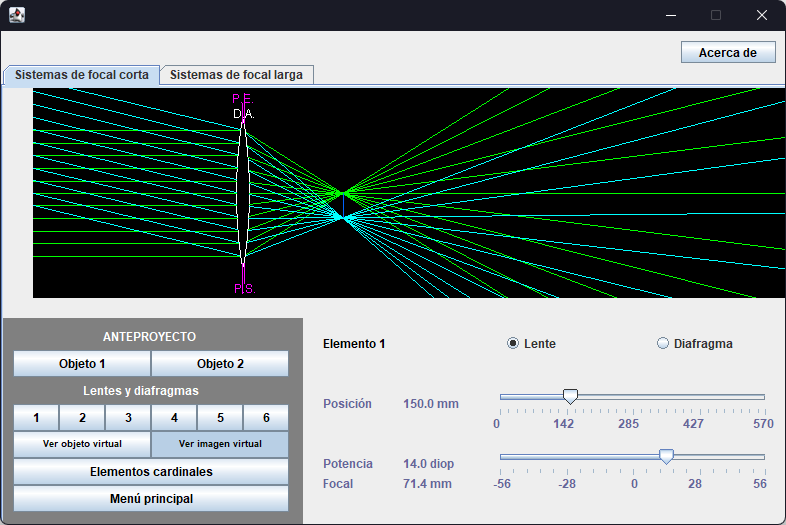
\includegraphics[width=0.49\textwidth]{fotos/parte 1/Lentes convergentes/convergentes_1_P14.png}
    \end{figure}
        
   \begin{wrapfigure}[9]{l}{0.5\textwidth}
        \vspace{-0.6cm}
        \centering
        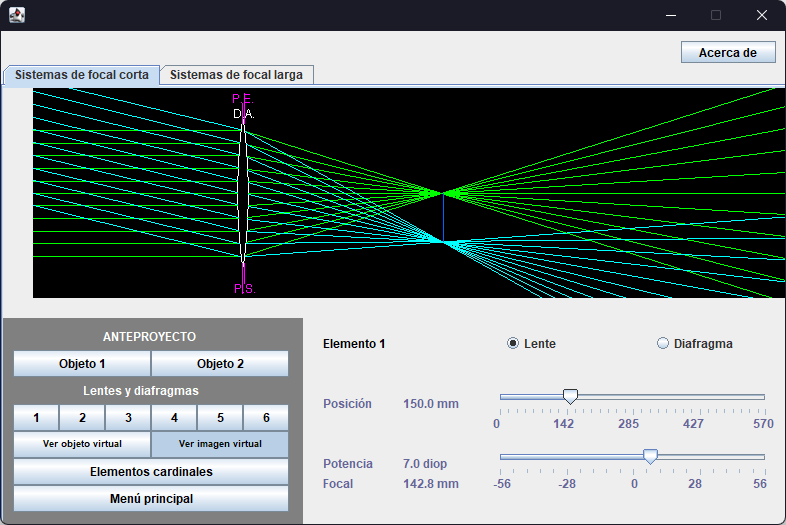
\includegraphics[width=0.49\textwidth]{fotos/parte 1/Lentes convergentes/convergentes_1_P7.png}
    \end{wrapfigure} 
    
    \noindent Las lentes elegidas tienen las siguientes potencias:\\

    $\begin{cases}
        \begin{aligned}
            &P_1 = 28\text{ D}\\
            &P_2 = 14\text{ D}\\
            &P_3 = 7\text{ D}
        \end{aligned}
    \end{cases}$\\

    \vspace{0.25cm}
    Se ve claramente cómo con la disminución de esta magnitud - que corresponde a un aumento en la distancia focal, puesto que $P = \frac{1}{f^\prime}$, la distancia del objeto a la lente va en aumento.
    
    \clearpage

    \noindent
    \textit{\textbf{CUESTIÓN 2.} Utilizando una lente positiva, diseña un sistema óptico que funcione como proyector y otro que funcione como lupa, en ambos casos objeto real, ¿dónde se ha de colocar el objeto con respecto al punto focal objeto de la lente en cada caso?}
    \\


   \begin{wrapfigure}[12]{l}{0.49\textwidth}
        \vspace{-0.55cm}
        \centering
        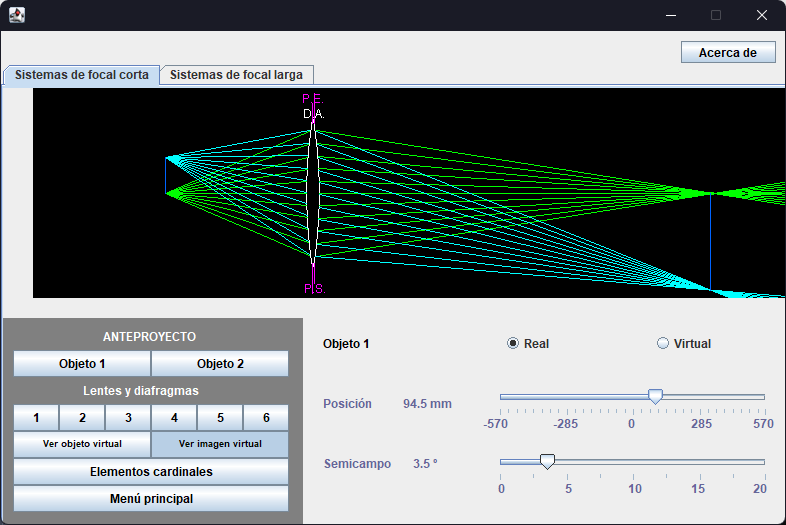
\includegraphics[width=0.49\textwidth]{fotos/parte 1/Lentes convergentes/convergentes_1_proyector.png}
        \label{fig:convergentes_2_proyector}
    \end{wrapfigure} 
    
    \noindent
    En un sistema que actúe como proyector, el aumento lateral será mayor a $1$, es decir, la imagen aparecerá más grande que el objeto. En este caso, tomando la posición del objeto bastante cercana a la lente ($s = -94.5\ mm$).\\
    
    \noindent Hemos empleado una lente convergente con potencia $P = 13\ D$, que nos proyectará una imagen de tamaño mayor al objeto, pero invertida.
    \hspace{0cm}\\\hspace{0cm}\\

    \begin{wrapfigure}[10]{r}{0.49\textwidth}
        \vspace{-0.55cm}
        \centering
        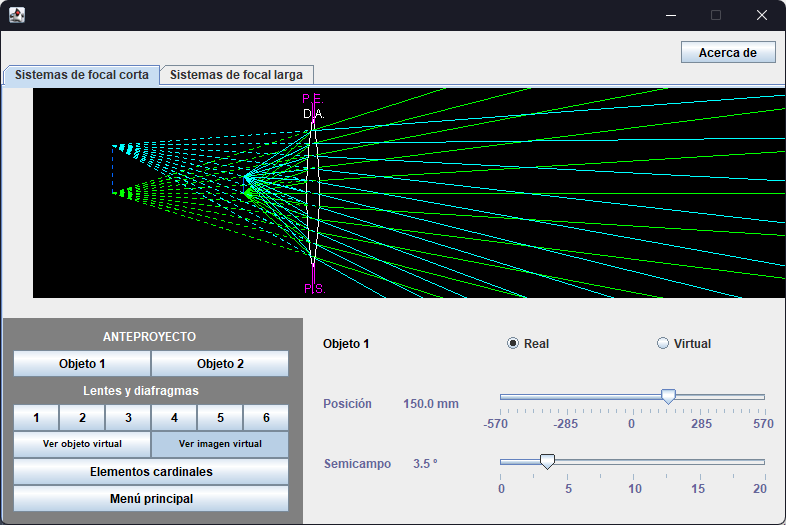
\includegraphics[width=0.49\textwidth]{fotos/parte 1/Lentes convergentes/convergentes_2_lupa.png}
        \label{fig:convergentes_2_lupa}
    \end{wrapfigure} 
    
    \noindent Ahora pasamos al caso de la lupa. Como queremos una imagen mayor al objeto en el espacio objeto, lo que haremos será poner nuestro objeto a la derecha de la lente\\

    \noindent Hemos tomado una lente exactamente igual a la del proyector, cambiando únicamente la posición del objeto, que ahora corresponde a $s = 150.0\ mm$. La imagen que se forma ahora es más grande y virtual.

    \clearpage
    \subsection{Lentes Divergentes}
        \subsubsection{Cuestiones previas}
        \vspace{0.2cm}
        \begin{wrapfigure}[9]{r}{0.5\textwidth}
            \vspace{-1.1cm}
            \centering
            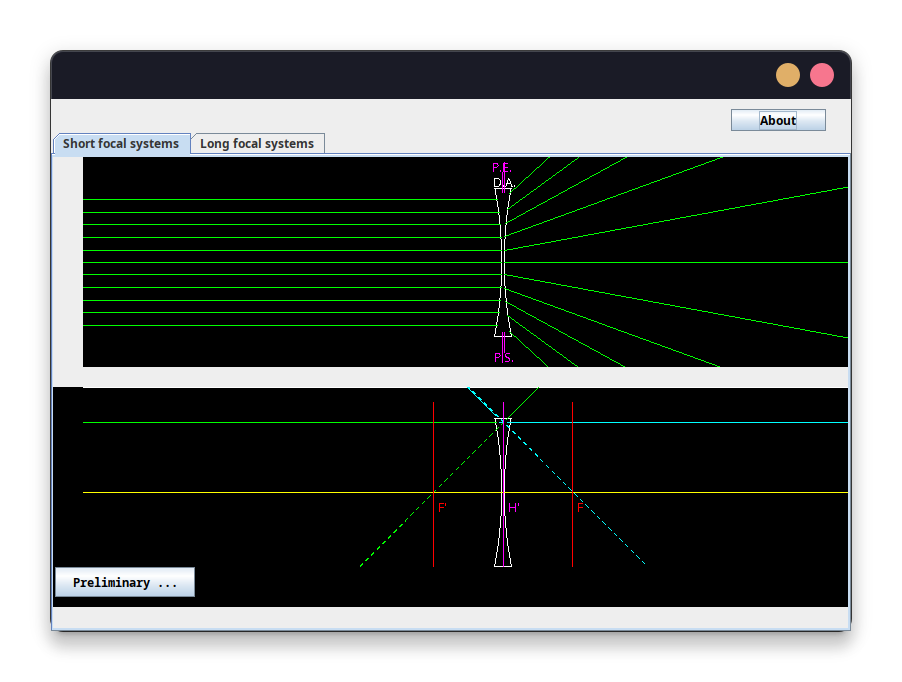
\includegraphics[width=0.51\textwidth]{fotos/parte 1/Lentes Divergentes/Cuestiones Previas/divergentes.png}
        \end{wrapfigure}
        
        \noindent Las cuestiones previas todas se realizaron alrededor de un sistema con las siguientes características:
        \begin{itemize}
            \item Lente de potencia $P = -20\ D$ en la posición $300.0\ mm$.
            \item Objeto real en infinito
        \end{itemize}
        
        Dicho sistema, junto con sus elementos cardinales, lo visualizamos en el programa \textit{UB Optics}.\hspace{0cm}\\\hspace{0cm}\\
        
        \textit{CUESTIÓN 1.  Modificar ahora la potencia de la lente negativa (-55.9 D, -28.0 D, -7.5D) y observar la trayectoria de los rayos para cada valor de potencia dado.}\\
        \vspace{0.5cm}Observamos cómo los rayos divergen más cuanto mayor es la potencia en valor absoluto.
        \begin{figure}[ht]
            \vspace{-0.8cm}
            \centering                
            \begin{subfigure}[t]{.49\textwidth}
                \centering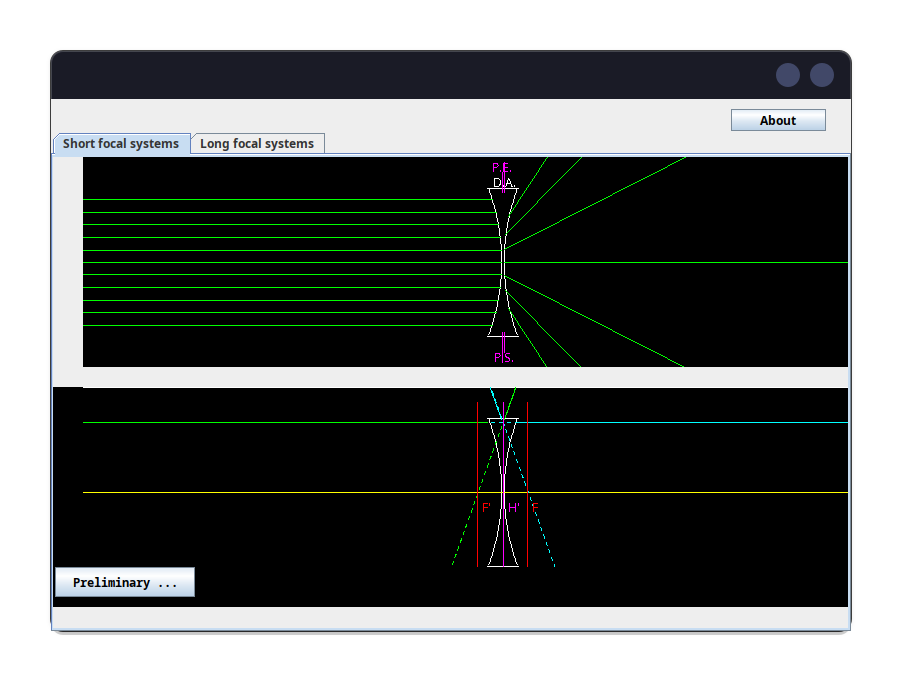
\includegraphics[width=\textwidth]{fotos/parte 1/Lentes Divergentes/Cuestiones Previas/559.png}
                \caption{Lente de potencia $-55.9\ D$}
            \end{subfigure}
            \begin{subfigure}[t]{.49\textwidth}
                \centering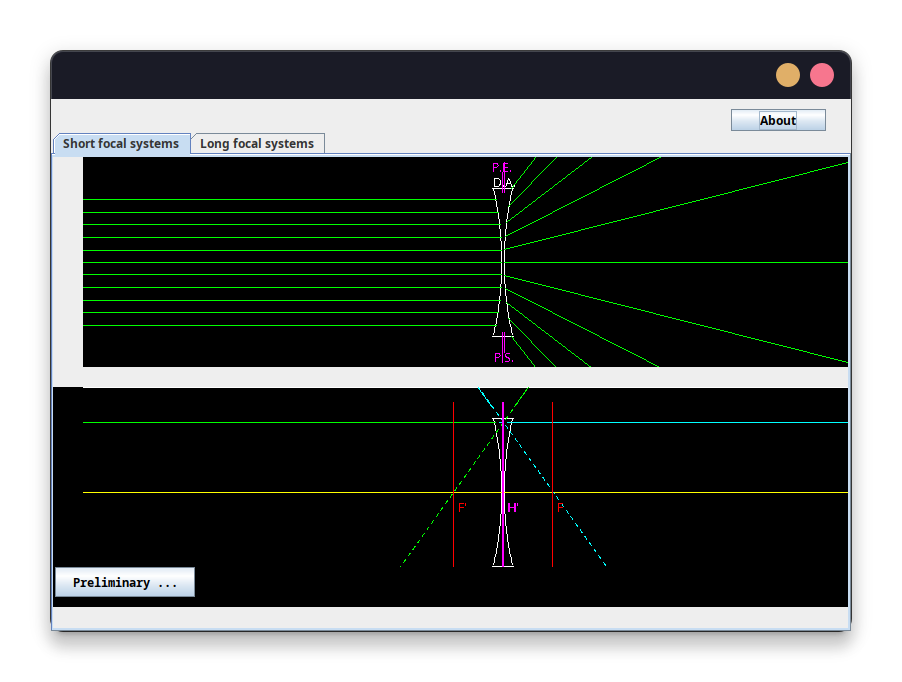
\includegraphics[width=\textwidth]{fotos/parte 1/Lentes Divergentes/Cuestiones Previas/280.png}
                \caption{Lente de potencia $-28.0\ D$}
            \end{subfigure}

            \begin{subfigure}[t]{.49\textwidth}
                \centering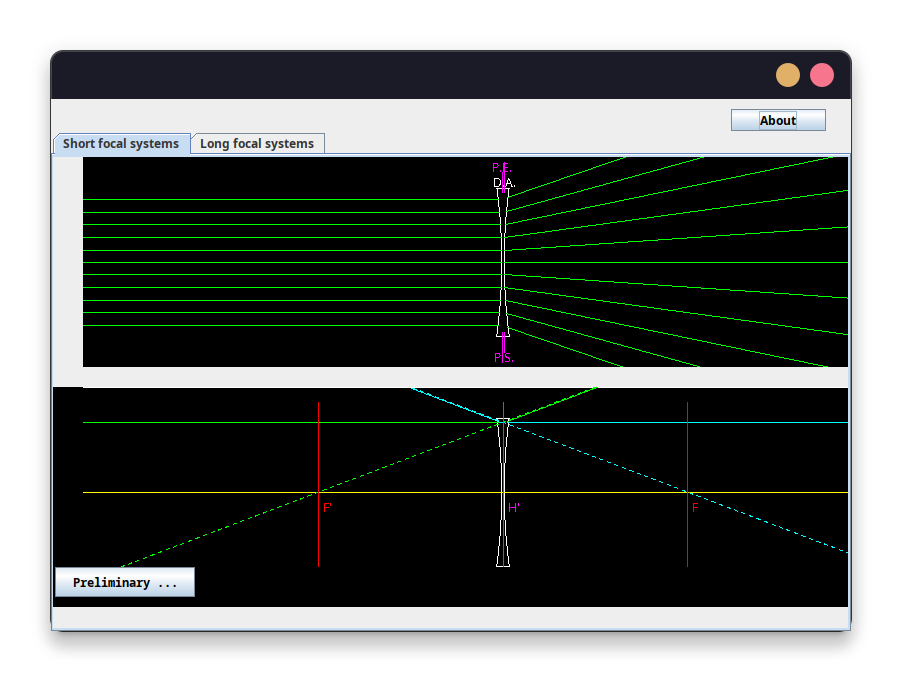
\includegraphics[width=\textwidth]{fotos/parte 1/Lentes Divergentes/Cuestiones Previas/75.png}
                \caption{Lente de potencia $-7.5\ D$}
            \end{subfigure}
        \end{figure}

        \clearpage
        \textit{CUESTIÓN 2.  Aproxima el objeto real a la lente inicial de $-20.0\ D$ con un semicampo de $3.7^\circ$, observa cómo se forma la imagen. ¿La imagen es derecha o invertida? ¿La imagen está aumentada o disminuida con respecto al tamaño del objeto? ¿Se puede situar el objeto en el foco objeto?}\\

        \begin{wrapfigure}[12]{l}{0.55\textwidth}
            \vspace{-1cm}
            \centering
            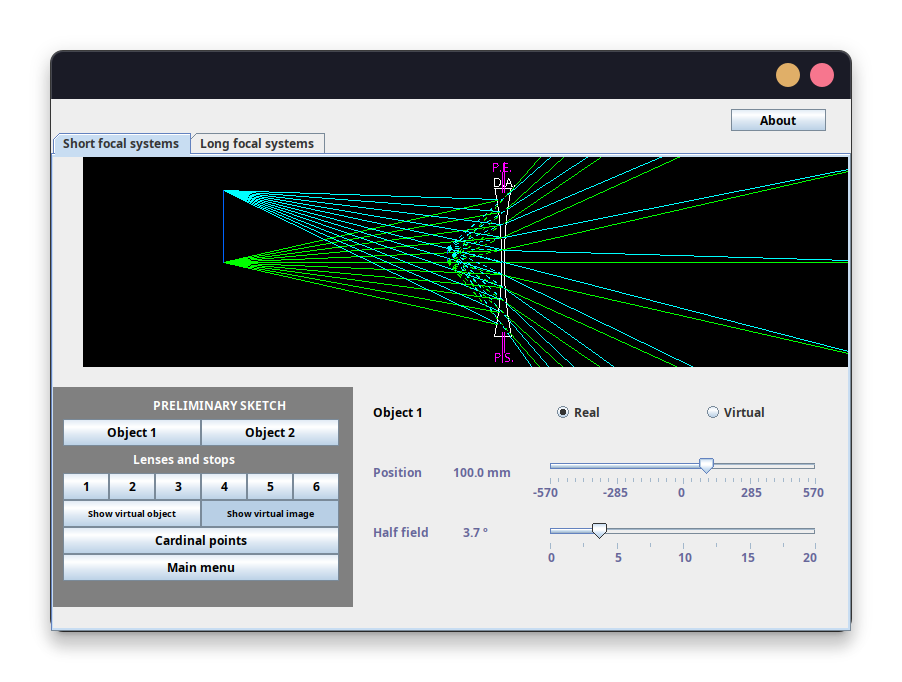
\includegraphics[width=0.56\textwidth]{fotos/parte 1/Lentes Divergentes/Cuestiones Previas/cuestionprevia2divergentes.png}
        \end{wrapfigure}

        \hspace{0mm}\\\hspace{0mm}Como podemos ver en la figura, la imagen es derecha y disminuida respecto al tamaño del objeto. Podemos situar el objeto en el foco objeto sin ningún problema.\\
        
        Vemos que al colocar el objeto en el foco objeto, la imagen se forma en el punto medio entre la lente y el foco, y está disminuida a la mitad. \\\hspace{0mm}\\\hspace{0mm}\\\hspace{0mm}\\\hspace{0mm}
            
        \textit{CUESTIÓN 3.  A continuación, vamos a hacer la simulación con un objeto virtual y semicampo $0^\circ$ (Objeto 1/virtual). Desactiva “ver imagen virtual” y activa “ver objeto virtual”. Desplaza el objeto virtual hasta situarlo en el foco objeto. ¿Qué sucede cuando el objeto virtual se sitúa en infinito?}\\

        \begin{wrapfigure}[10]{r}{0.55\textwidth}
            \vspace{-1.1cm}
            \centering
            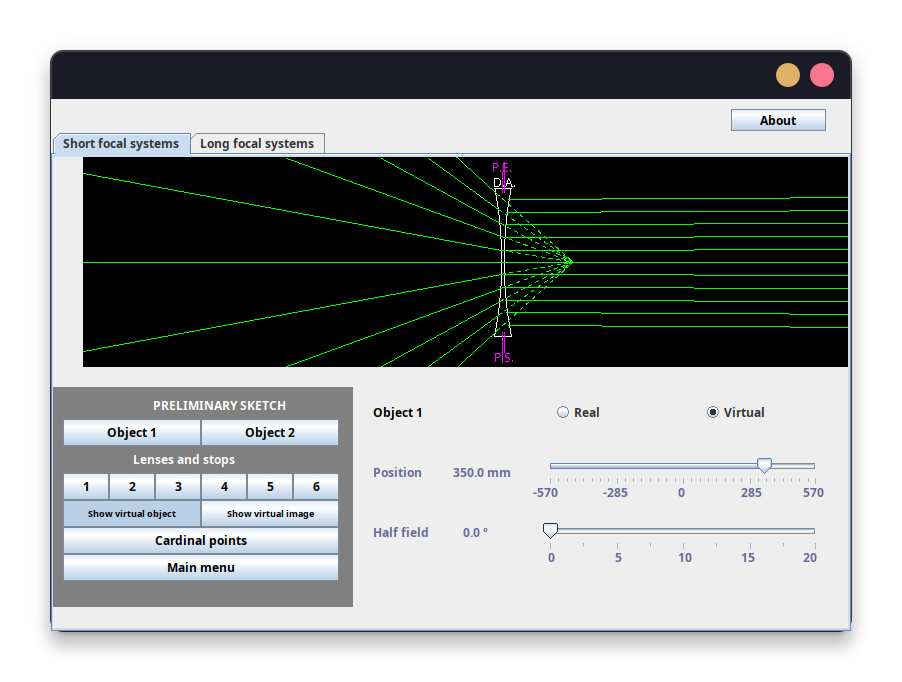
\includegraphics[width=0.56\textwidth]{fotos/parte 1/Lentes Divergentes/Cuestiones Previas/screenshot.png}
        \end{wrapfigure}
        
        \hspace{0mm}\\\hspace{0mm}\\\hspace{0mm}\\En la figura vemos cómo al situar el objeto en el foco objeto, la imagen se forma en el infinito. Sin embargo, al situar el objeto en el infinito la imagen se forma en el foco imagen.\\\hspace{0mm}\\\hspace{0mm}\\\hspace{0mm}\\\hspace{0mm}\\\hspace{0mm}\\
        
        \textit{CUESTIÓN 4.  Visualizar los elementos cardinales de este sistema}\\

        \begin{figure}[ht]
            \centering
            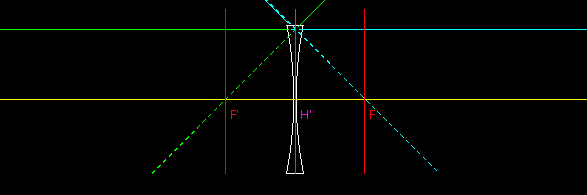
\includegraphics[width=0.6\textwidth]{fotos/parte 1/Lentes Divergentes/Cuestiones Previas/cardinales.png}
        \end{figure}
        
        \clearpage
        \subsubsection{Cuestiones propuestas}
        \textit{\textbf{CUESTIÓN 3.} Comprobar con una lente divergente que para todas las posiciones de objeto real (semicampo 3.5°) la imagen es de menor tamaño, mientras que cuando el objeto es virtual el tamaño de la imagen aumenta. Represéntalo para dos posiciones cuales quiera del objeto real y dos posiciones del objeto virtual ( $s<f\ $ y $\ s>f$ ) ¿Las imágenes son derechas o invertidas?}\\
        
        Vamos a comprobar qué sucede en un sistema con una lente divergente de $-8.0$ D, focal a $-125$ mm y con semicampo $3.5^\circ$ cuando situamos un objeto real antes y después de dicha distancia focal: Las imágenes son derechas y virtuales, además, la imagen es de menor tamaño que el objeto.

        \begin{figure}[ht]
            \centering
            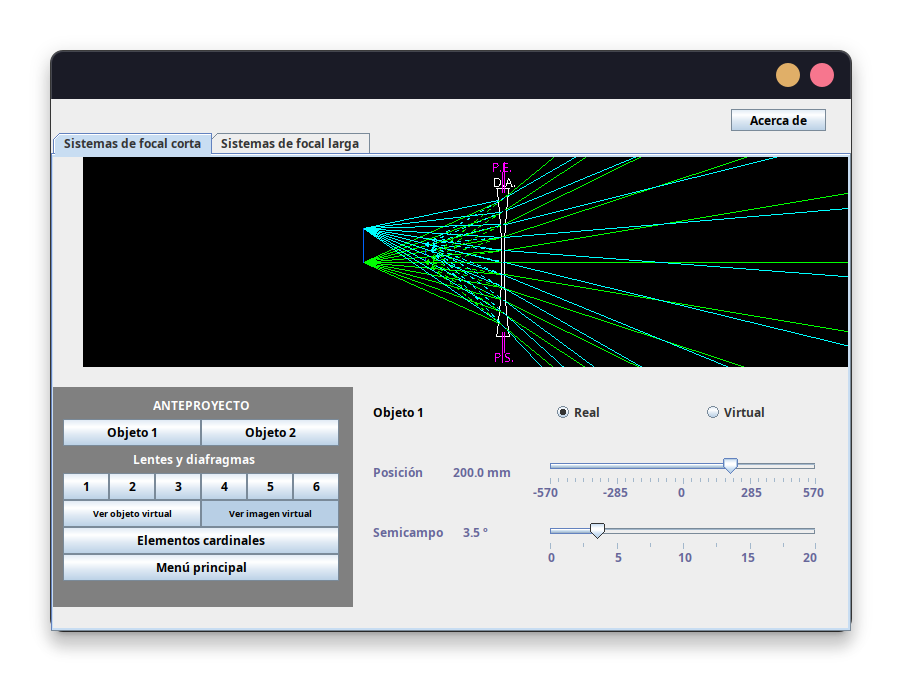
\includegraphics[width=0.49\textwidth]{fotos/parte 1/Lentes Divergentes/Cuestión Propuesta/1.3.Real.Antes.png}
            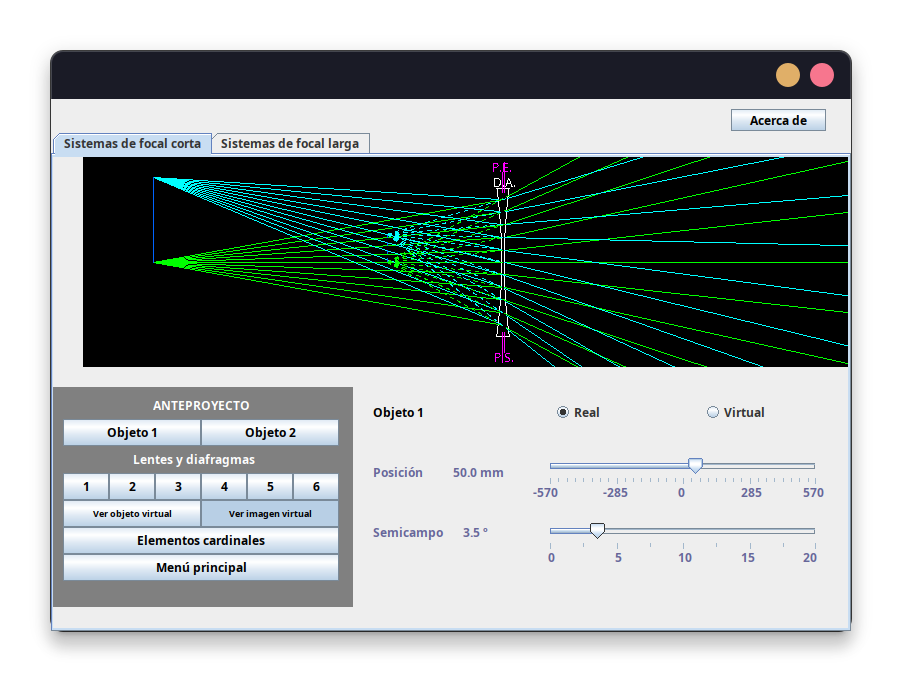
\includegraphics[width=0.49\textwidth]{fotos/parte 1/Lentes Divergentes/Cuestión Propuesta/1.3.Real.Despues.png}
        \end{figure}

        \noindent Tratamos ahora el caso en el que el objeto es real, y vemos qué pasa cuando lo situamos antes y después de la distancia focal: Las imágenes son reales e invertidas, además, la imagen es de mayor tamaño que el objeto. Es el caso opuesto al anterior.

        \begin{figure}[ht]
            \centering
            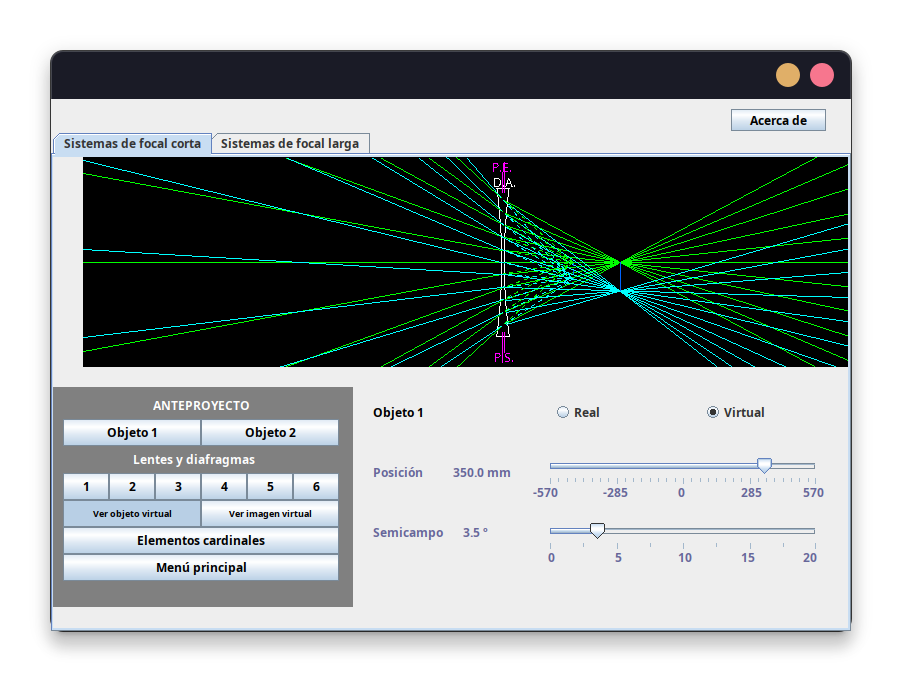
\includegraphics[width=0.49\textwidth]{fotos/parte 1/Lentes Divergentes/Cuestión Propuesta/1.3.Virtual.Antes.png}
            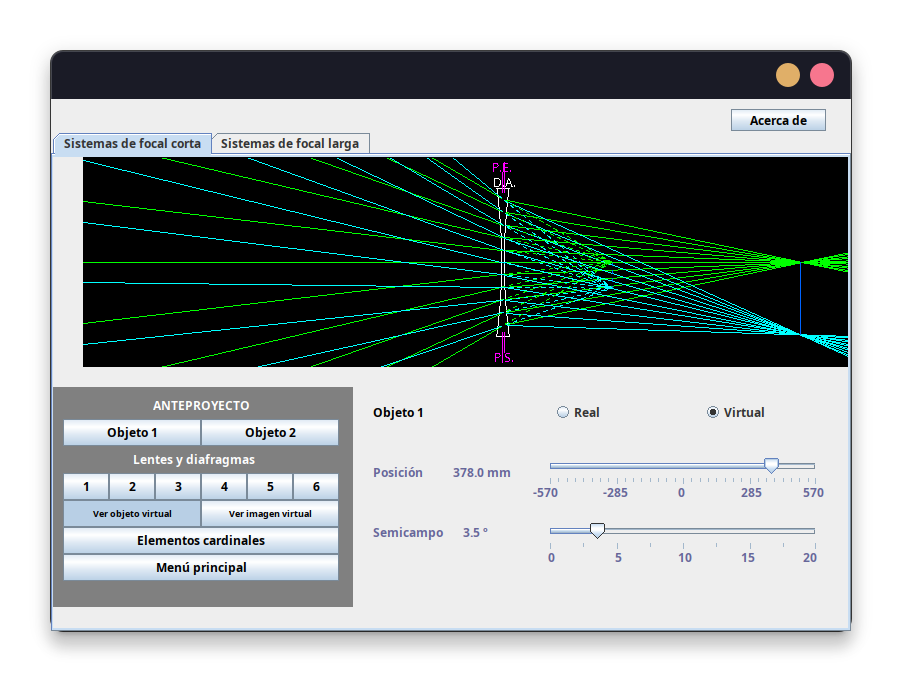
\includegraphics[width=0.49\textwidth]{fotos/parte 1/Lentes Divergentes/Cuestión Propuesta/1.3.Virtual.Despues.png}
        \end{figure}

    \newpage

    \vspace{-0.5cm}\subsection{Aberraciones Ópticas}
        \subsubsection{Aberración Esférica}
            %4- Calcular el factor de forma que minimiza la aberración esférica teórica y experimentalmente para n=1,5 y comprobar que el factor de forma que corresponde a los radios extremos para esta posición del objeto genera mayor aberración.
            \textit{\textbf{CUESTIÓN 4.} Calcular el factor de forma que minimiza la aberración esférica teórica y experimentalmente para n=1,5 y comprobar que el factor de forma que corresponde a los radios extremos para esta posición del objeto genera mayor aberración.}\\

            Vamos a calcular el factor de forma $q$ que minimiza y maximiza la aberración esférica para una lente de $10$D, focal $f^\prime=100$mm y $n=1.5$ para un objeto situado en el infinito. Para ello, hemos de derivar e igualar a cero:

            \begin{equation}
                A = \dfrac{1}{s^\prime_h}-\dfrac{1}{s^\prime_p}=\dfrac{h^2}{8{f^\prime}^3}\dfrac{1}{n(n-1)}\left(\dfrac{n+2}{n-1}q^2+4(n+1)pq+(3n+2)(n-1)p^2+\dfrac{n^3}{n-1}\right)
                \label{eq:AberracionEsferica}
            \end{equation}

            \begin{equation}
                \dfrac{\partial A}{\partial q}=\dfrac{h^2}{8 {f^\prime}^3}\dfrac{1}{n(n-1)}\left(2\dfrac{n+2}{n-1}q+4(n+1)p\right)=0
                \label{eq:DerivadaAberracion}
            \end{equation}
            
            Y así obtenemos finalmente una fórmula nos da el factor de forma $q$ en función de $n$ y de $p$ que minimiza la aberración esférica de nuestro sistema.

            \begin{equation}
                q=\dfrac{-4(n+1)(n-1)}{2(n+2)}p
                \label{eq:AberracionEsfericaMinima}
            \end{equation}\\

            Para nuestro sistema, podemos decir que $p=-1$ ya que el objeto está en el infinito, y como tenemos que $n=1.5$, podemos obtener teóricamente que el valor de $q$ que minimiza la aberración esférica es $q=0.714$. \\
            
            \begin{wrapfigure}[14]{l}{0.55\textwidth}
                \vspace{-0.8cm}
                \centering
                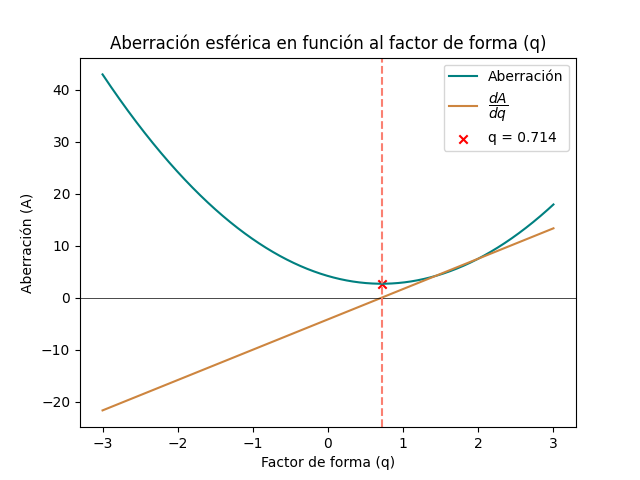
\includegraphics[width=0.58\textwidth]{fotos/parte 1/Aberraciones/Aberración Esférica/factor_de_forma.png}
            \end{wrapfigure}
            
            \hspace{0cm}\\Vamos a usar un código que genera gráficas en python para corroborar experimentalmente este dato. Dicho código se encuentra en el anexo.\\

            Graficamos la aberración en función del factor de forma, así como su derivada respecto a $q$. Calculamos el valor mínimo de la aberración y vemos que el valor de $q$ coincide con el punto de corte de la derivada con el eje x.\\\hspace{0cm}\\
            
            Como podemos ver en dicha figura, el valor de $q$ que minimiza la aberración esférica es el mismo que hemos calculado analíticamente.\\

            \clearpage
            También vamos a corroborar este resultado mediante el uso del programa \textit{UB Optics}. Bajo la pestaña de \textit{Exact Ray Tracing / Image} hemos de jugar con la escala para hacer visible este mínimo. Como podemos ver en las imágenes, la posición que más se acerca al factor de forma calculado es la que tiene los círculos más concéntricos. Es algo difícil de apreciar en las imágenes, pero en el programa se ve claramente que el segundo caso es el mínimo, y es el que más se acerca al factor calculado analíticamente. 

            \begin{figure}[ht]
                \centering
                \begin{subcaptionblock}{.333\textwidth}
                    \centering
                    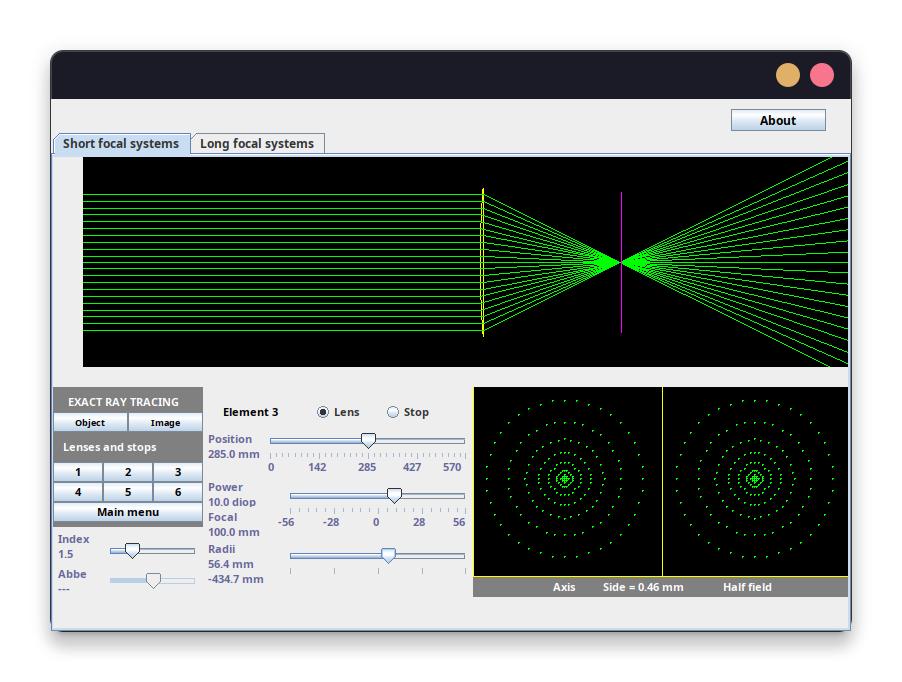
\includegraphics[width=\textwidth]{fotos/parte 1/Aberraciones/Aberración Esférica/abbEsf56.png}
                    \caption{$q=0.77$}
                \end{subcaptionblock}%                
                \begin{subcaptionblock}{.333\textwidth}
                    \centering
                    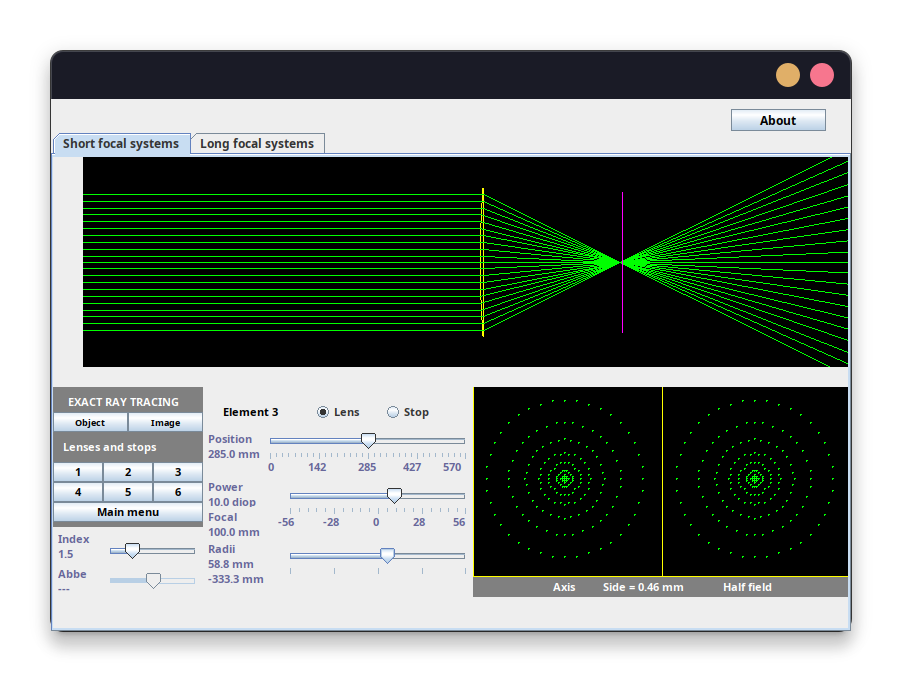
\includegraphics[width=\textwidth]{fotos/parte 1/Aberraciones/Aberración Esférica/abbEsf58.png}
                    \caption{$q=0.7$}
                \end{subcaptionblock}%                
                \begin{subcaptionblock}{.333\textwidth}
                    \centering
                    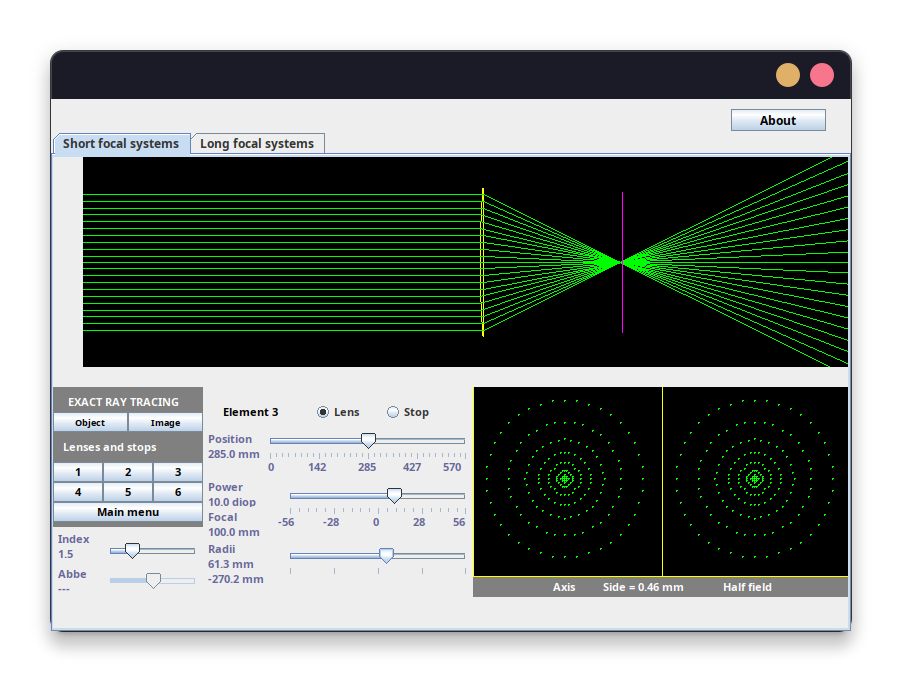
\includegraphics[width=\textwidth]{fotos/parte 1/Aberraciones/Aberración Esférica/abbEsf61.png}
                    \caption{$q=0.77$}
                \end{subcaptionblock}    
                \caption{Cálculo experimental del factor de forma}
            \end{figure}
            \begin{figure}[ht]
                \centering
                \begin{subcaptionblock}{.333\textwidth}
                    \centering
                    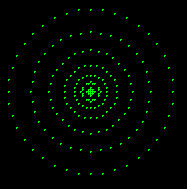
\includegraphics[width=\textwidth]{fotos/parte 1/Aberraciones/Aberración Esférica/52.png}
                    \caption{$q=0.77$}
                \end{subcaptionblock}%                
                \begin{subcaptionblock}{.333\textwidth}
                    \centering
                    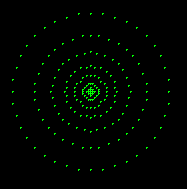
\includegraphics[width=\textwidth]{fotos/parte 1/Aberraciones/Aberración Esférica/58.png}
                    \caption{$q=0.7$}
                \end{subcaptionblock}%                
                \begin{subcaptionblock}{.333\textwidth}
                    \centering
                    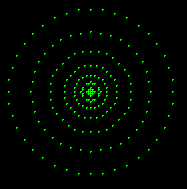
\includegraphics[width=\textwidth]{fotos/parte 1/Aberraciones/Aberración Esférica/67.png}
                    \caption{$q=0.77$}
                \end{subcaptionblock}    
                \caption{Cálculo experimental del factor de forma (zoom)}
            \end{figure}
            
            \textit{\textbf{CUESTIÓN 5.} ¿Se mantiene la misma aberración esférica al modificar la posición del objeto, por ejemplo, al situar el objeto a dos veces la focal (2f)? ¿Cuál será el q mínimo experimental en este caso? Modificar la posición de la lente a 200mm para visualizar mejor la imagen.}\\

            Puesto que ahora el objeto ya no está en el infinito, el valor de $p$ ya no es $-1$ y por tanto variará el valor obtenido para $q$. Para ello, hemos de calcular $p$ mediante:
            \begin{equation}
                \dfrac{s^\prime+s}{s^\prime-s}=\dfrac{2f^\prime + 2f}{2f^\prime - 2f}=\dfrac{200-200}{200+200}=0
                \label{eq:p}
            \end{equation}
            Como podemos observar, ahora el valor de $p$ pasa a ser cero.
            
            \clearpage
            Si sustituimos el nuevo valor de $p$ en la ecuación \ref{eq:AberracionEsfericaMinima} obtenemos que el nuevo factor de forma que minimiza la aberración esférica es $q=0$.\\
            
            Usando otra vez el mismo código de \textit{python} y el programa \textit{UB Optics} vemos como este resultado concuerda con lo observado experimentalmente. Python nos devuelve que $q=0$ y nuevamente en el programa observamos como los círculos más concéntricos aparecen cuando no modificamos la curvatura de las lentes.
            
            \begin{figure}[ht]
                \centering
                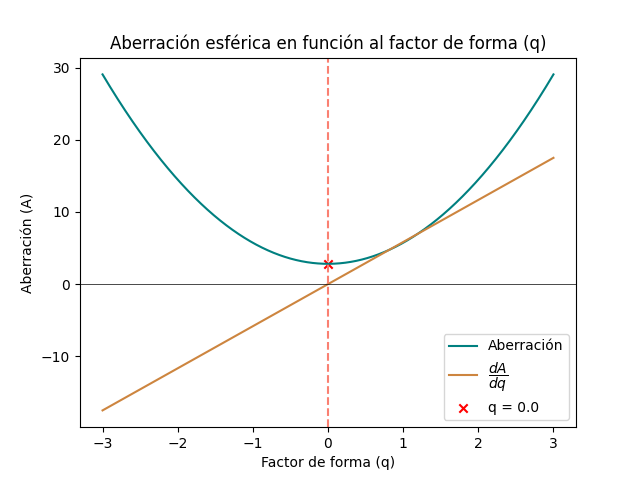
\includegraphics[width=0.49\textwidth]{fotos/parte 1/Aberraciones/Aberración Esférica/factor_de_forma_2f.png}
                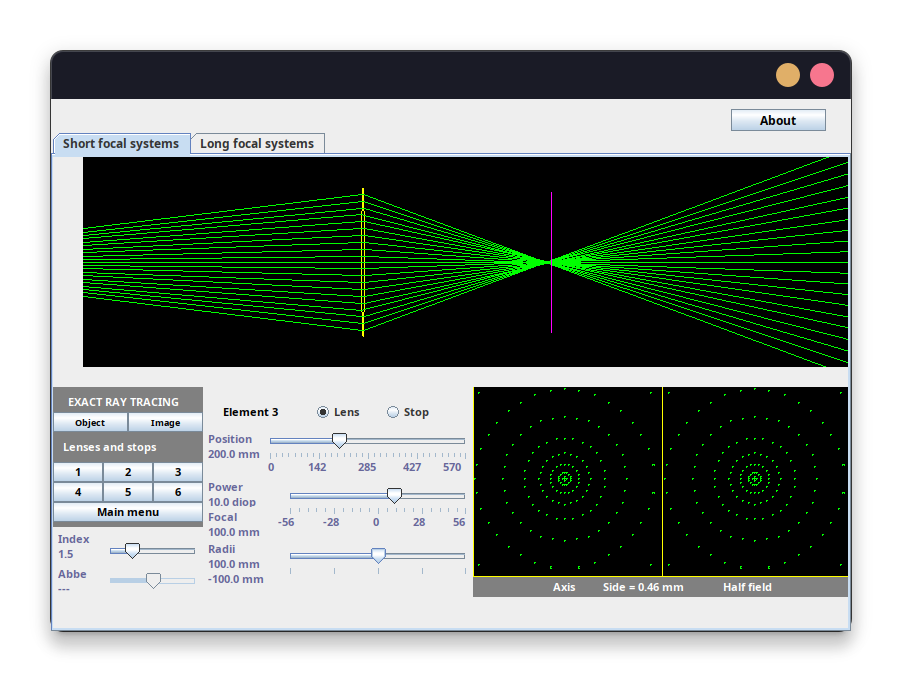
\includegraphics[width=0.49\textwidth]{fotos/parte 1/Aberraciones/Aberración Esférica/AbEsf_2f.png}
            \end{figure}

        \vspace{-0.5cm}
        \subsubsection{Coma}
        \textit{\textbf{CUESTIÓN 6.} Calcular el factor de forma que anula esta aberración teórica y experimentalmente. Comprueba que al cambiar la posición de la imagen a 0 mm el factor de forma experimental es único.} \\
        
        \begin{wrapfigure}[6]{r}{0.5\textwidth}
            \vspace{-0.5cm}
            \centering
            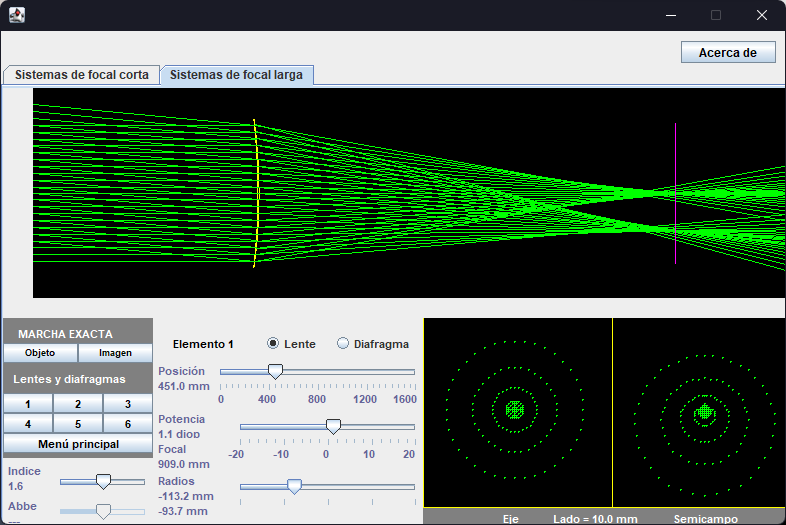
\includegraphics[width=0.49\textwidth]{fotos/parte 1/Aberraciones/aberraciones_6_montaje.png}
            \label{fig:aberraciones_6_montaje}
        \end{wrapfigure}
        \noindent Lo primero que haremos será montar el sistema tal y como se nos indica en el informe.
        \begin{itemize}
            \item Lente de potencia $P = 1.1\ D$ y radios $r_1 = -113.2\ mm$, $r_2 = -93.7 mm$, situada en la posición $451.0\ mm$.
            \item Objeto situado en el infinito con semicampo de $1.3^\circ$.
        \end{itemize}
        \vspace{18mm}
        \noindent Tomando la imagen a $s' = -46\ mm$ del plano paraxial, lo que nos queda es lo siguiente:
        
        \noindent Se ve un coma muy pronunciado que queremos minimizar.
        
        \clearpage 
        De forma gráfica, veremos que alcanza su valor mínimo para $r_1 = 521.7\ mm$ y $r_2 = 11999.9\ mm$:
        \begin{figure}[ht]
            \centering
            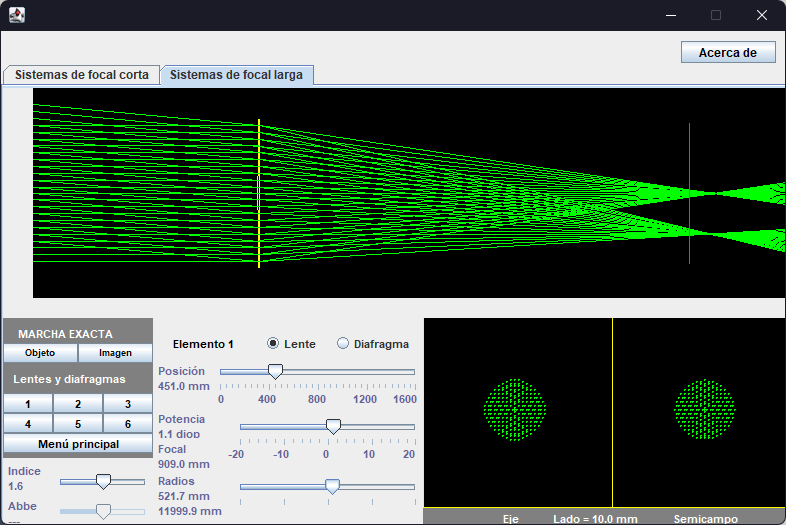
\includegraphics[width=0.4\textwidth]{fotos/parte 1/Aberraciones/Aberración Esférica/coma_min_nuevo.png}
            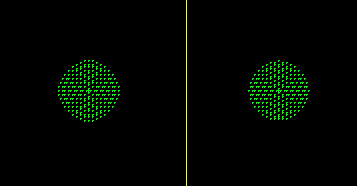
\includegraphics[width=0.5\textwidth]{fotos/parte 1/Aberraciones/Aberración Esférica/coma_min_nuevo (1).png}
        \end{figure}
            
        Para estos datos, el factor de forma queda:
        \begin{equation*}
            q = \frac{r_2 + r_1}{r_2 - r_1}\ \Longrightarrow q = \frac{11999.9 + 521.7}{11999.9 - 521.7} = 1.09
        \end{equation*}
        \\
        \noindent Vamos a ver cómo obtener este mismo resultado de forma analítica. Para ello, partimos de la ecuación que nos define el coma:
        \begin{equation}
            c_s = \frac{y'h^2}{f'^2}\left[\frac{3(2n+1)}{4n}p + \frac{3(n+1)}{4n(n-1)}q\right]
        \end{equation}
        \noindent
        Si igualamos esta expresión a 0, hallaremos el valor del parámetro $q$ que lo anula.
        \begin{equation*}
            c_s = \frac{y'h^2}{f'^2}\left[\frac{3(2n+1)}{4n}p + \frac{3(n+1)}{4n(n-1)}q\right]= 0\Longleftrightarrow \frac{3(2n+1)}{4n}p + \frac{3(n+1)}{4n(n-1)}q = 0
        \end{equation*}
        \\
        \noindent Para resolver esta ecuación, primero hemos de obtener el valor del factor de posición $p$ cuando $s \rightarrow \infty$:
        \begin{equation*}
            \lim_{s \to \infty}p=\lim_{s \to \infty}\frac{s' + s}{s'-s}= \lim_{s \to \infty}\frac{\sfrac{s'}{s} + 1}{\sfrac{s'}{s}-1} = \frac{1}{-1} = -1
        \end{equation*}
        \begin{equation*}
            \frac{3(2n+1)}{4n}p + \frac{3(n+1)}{4n(n-1)}q = -\frac{3(2n+1)}{4n} + \frac{3(n+1)}{4n(n-1)}q = 0 \Longleftrightarrow q = \frac{(2n+1)(n-1)}{(n+1)} = 0.97
        \end{equation*}
        \\
        \noindent Vemos que el factor de forma calculado analíticamente toma un valor muy similar al experimental. Solo nos queda ver qué es lo que ocurre cuando cambiamos la posición de la imagen a $s' = 0mm$:
        
        \begin{figure}[ht]
            \centering
            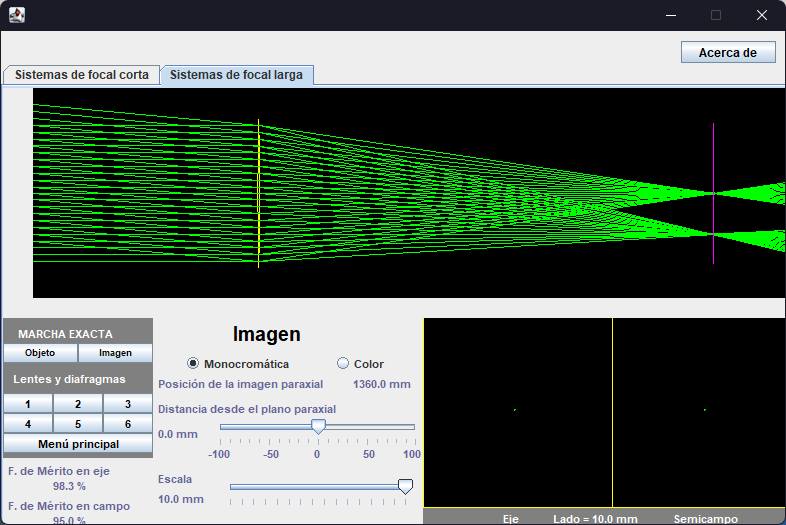
\includegraphics[scale = 0.35]{fotos/parte 1/Aberraciones/aberraciones_6_coma_0mm.png}
            \label{fig:aberraciones_6_coma_0mm}
        \end{figure}

        \noindent En este caso el coma es prácticamente nulo, y por tanto la imagen que se producirá se verá con total nitidez.
    
\clearpage
\section{Diseño y estudio de instrumentos ópticos}
    \vspace{-0.2cm}
    \subsection{Cuestiones previas}
    \noindent Antes de empezar con las cuestiones propuestas, vamos a estudiar las preguntas 1) y 2) de las no propuestas (puesto que las demás coinciden se solapan con las relativas al anteojo).
    \\
    \noindent Primero vamos a proponer un sistema con las siguientes características:
    \begin{itemize}
        \item Lente de potencia $P = 5\ D$ a $100\ mm$.
        \item Diafragma de diámetro $\varnothing = 14.7\ mm$ en la posición $300\ mm$.
        \item Lente de potencia $P = 20\ D$ separada de la primera lente $250\ mm$.
        \item Objeto en infinito con un semicampo de $2^o$.
    \end{itemize}
    \vspace{0.2cm}
    \textit{CUESTIÓN 1. Visualizar los elementos cardinales de sistema* y las pupilas de entrada y salida del sistema. Observa la orientación de la imagen final. Las líneas azules permiten determinar H y las verdes H’. Observa que la situación óptima en la que no exista viñeteado implica la colocación de un diafragma en la imagen intermedia.}
    \\
    
    \begin{wrapfigure}[11]{l}{0.49\textwidth}
                \vspace{-0.54cm}
                \centering
                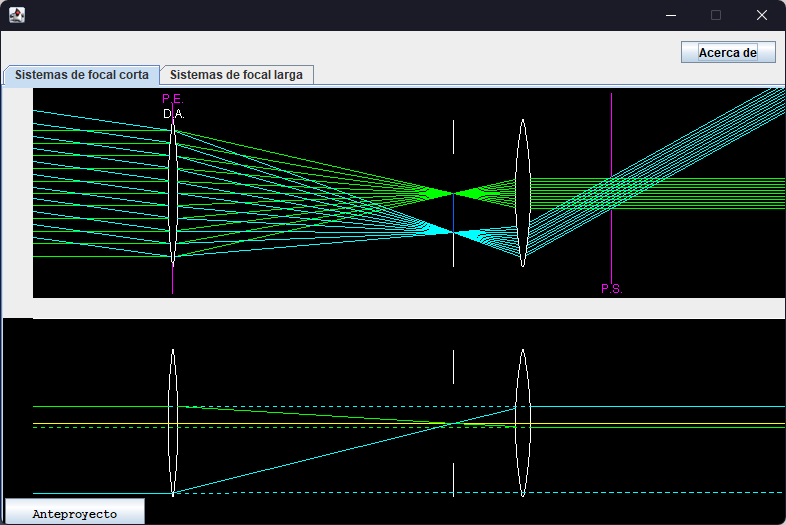
\includegraphics[width=0.48\textwidth]{fotos/parte 2/No negrita/no_propuesta_1.png}
            \end{wrapfigure}
    \noindent Los elementos cardinales del sistema son los que se muestran a continuación:\\ 
    
    \noindent En la imagen superior queda indicado que tanto pupila de entrada (PE) como diafragma de apertura (DA) son la primera lente, mientras que la pupila de salida (PS) corresponde a la imagen de esta a través de la segunda lente. En cuanto a los planos principales H y H', por las líneas azules y verdes trazadas en la figura inferior vemos que coinciden con las lentes.\\
    
    
    \textit{CUESTIÓN 2. Construir un anteojo terrestre con sistema inversor simple, $f^\prime_1 = 100\ mm$; $f^\prime_2 = f^\prime_{SI} = 50\ mm$. Posición de la lente 1: $50 mm$.}    
    \noindent Al construir el anteojo nos queda el siguiente sistema:
    \begin{figure}[ht]
        \centering
        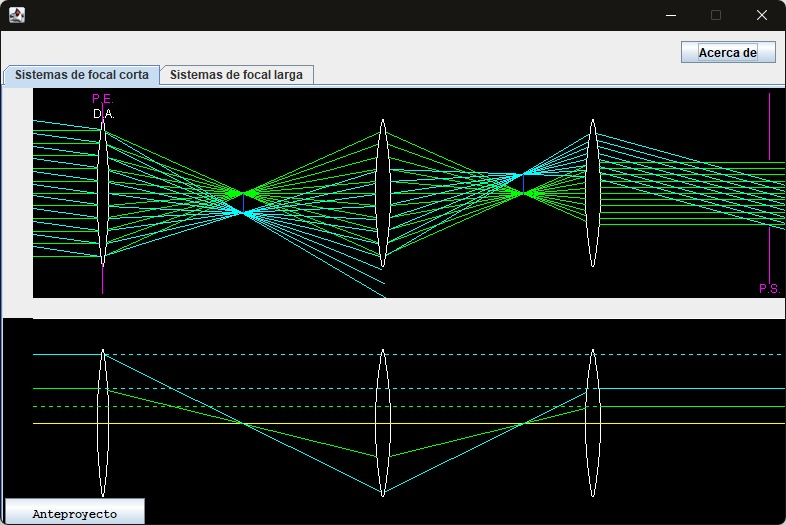
\includegraphics[width=0.53\textwidth]{fotos/parte 2/No negrita/no_propuesta_2.jpeg}
    \end{figure}

    \clearpage
    \subsection{Anteojo}
        \textit{\textbf{CUESTIÓN 7.} Construir un anteojo con sistema inversor doble $f^\prime_A = f^\prime_B = 50\ mm$}\\

            \begin{wrapfigure}[9]{l}{0.49\textwidth}
                \vspace{-1cm}
                \centering
                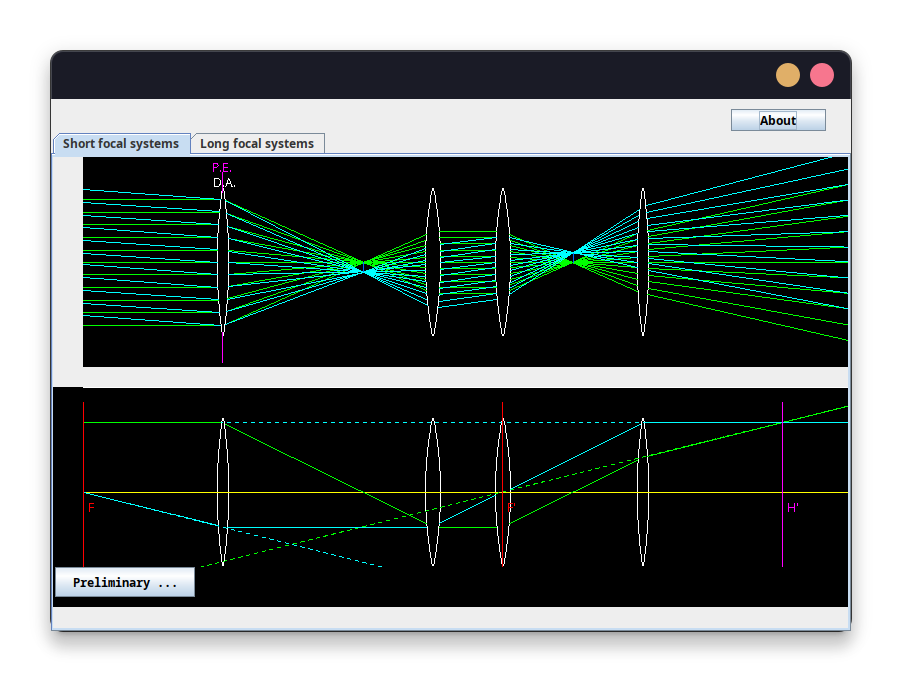
\includegraphics[width=0.51\textwidth]{fotos/parte 2/Anteojo/cuestion7.png}
            \end{wrapfigure}

            Para esta cuestión hemos de colocar los siguientes datos en el programa:
            \begin{itemize}
                \item (1) Lente de $10\ D$ en $100\ mm$.
                \item (A) Lente de $20\ D$ en $250\ mm$.
                \item (B) Lente de $20\ D$ en $300\ mm$.
                \item (2) Lente de $10\ D$ en $400\ mm$.
            \end{itemize}
            El objeto se situó en el infinito con un semicampo de $2^\circ$.\\
            
            Como vemos en la figura, la focal objeto de la lente A coincide con la focal imagen de la lente 1. Además la focal imagen de la lente B coincide con la focal objeto de la lente 2. \\
            
        \vspace{0.4cm}
        \textit{\textbf{CUESTIÓN 8.} Construir un anteojo de Galileo utilizando una lente de $-20.0\ D$.}\\
        
        \begin{wrapfigure}[8]{r}{0.49\textwidth}
                \vspace{-1cm}
                \centering
                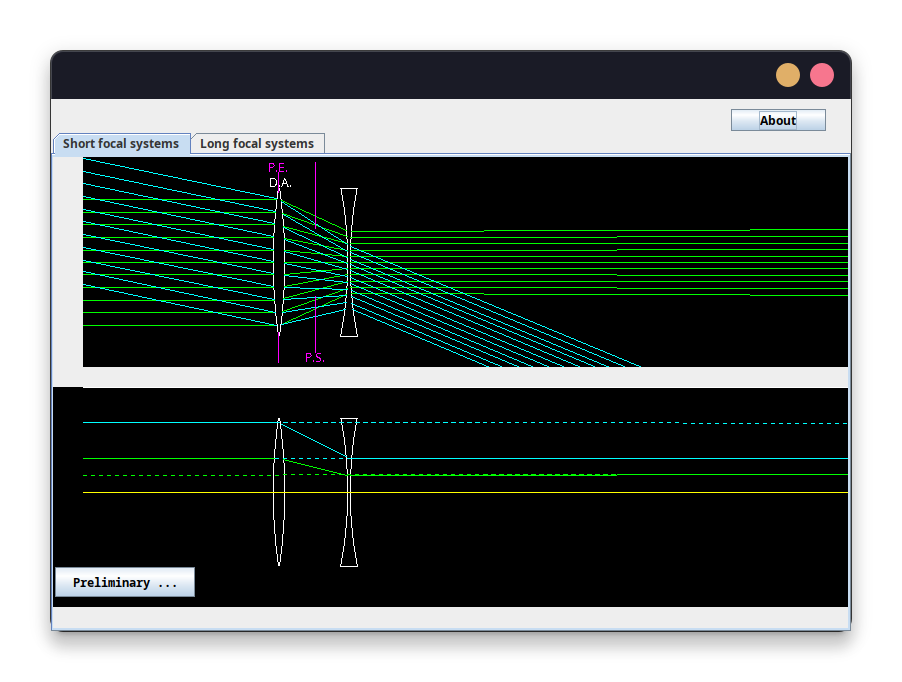
\includegraphics[width=0.51\textwidth]{fotos/parte 2/Anteojo/galileo.png}
        \end{wrapfigure}

        Para hacer un anteojo de Galileo hemos de construir un sistema tal que la distancia entre las lentes sea $f^\prime_1 - f_2$. En nuestro caso, calculamos la separación y obtenemos un valor de $50\ $mm. Por tanto:
        \begin{itemize}
            \item Lente de $10\ $D en $140\ $mm
            \item Lente de $-20\ $D en $190\ $mm
        \end{itemize}
        El objeto se situó en el infinito con un semicampo de $3^\circ$.\\

        \vspace{0.4cm}
        \textit{\textbf{CUESTIÓN 9.} Compara los elementos cardinales y las pupilas de entrada y salida de este sistema óptico con los de los sistemas anteriores. Observa la orientación de la imagen final en este caso.}\\

        Para realizar esta cuestión, hemos de fijarnos en la parte inferior del programa en las figuras de las cuestiones no propuestas 1 y 2 así como de las cuestiones propuestas 7 y 8.\\
        
        Así, vemos que los cuatro sistemas tienen los elementos cardinales en el infinito. También tienen en común que la pupila de entrada (PE) es la primera lente. Sin embargo, la pupila de salida (PS) está detrás de todas las lentes para todos los sistemas menos el anteojo de Galileo, donde la PS está entre las lentes.\\
        
        \clearpage
        Para observar la orientación de la imagen final respecto al objeto vamos a estudiar el signo de $\Gamma$. 

        \begin{table}[ht]
            \centering
            \begin{tabular}{c|c|c|c|c|}
                \cline{2-5}
                \textbf{} &
                  \cellcolor[HTML]{010066}{\color[HTML]{FFFFFF} \textbf{\begin{tabular}[c]{@{}c@{}}Anteojo \\ astronómico\end{tabular}}} &
                  \cellcolor[HTML]{010066}{\color[HTML]{FFFFFF} \textbf{\begin{tabular}[c]{@{}c@{}}Anteojo terrestre \\ simple\end{tabular}}} &
                  \cellcolor[HTML]{010066}{\color[HTML]{FFFFFF} \textbf{\begin{tabular}[c]{@{}c@{}}Anteojo terrestre \\ doble\end{tabular}}} &
                  \cellcolor[HTML]{010066}{\color[HTML]{FFFFFF} \textbf{\begin{tabular}[c]{@{}c@{}}Anteojo \\ de Galileo\end{tabular}}} \\ \hline
                \rowcolor[HTML]{EFEFEF} 
                \multicolumn{1}{|c|}{\cellcolor[HTML]{EFEFEF}\textbf{Signo de $\Gamma$}} &
                  $<0$ &
                  $>0$ &
                  $>0$ &
                  $>0$ \\
                \rowcolor[HTML]{FFFFFF} 
                \multicolumn{1}{|c|}{\cellcolor[HTML]{FFFFFF}\textbf{\begin{tabular}[c]{@{}c@{}}Imagen\end{tabular}}} &
                  Invertida &
                  Derecha &
                  Derecha &
                  Derecha \\ \hline
            \end{tabular}
            \label{table:cuestion9}
        \end{table}

        \vspace{0.4cm}
        \textit{\textbf{CUESTIÓN 10.} Calcula el aumento visual de los anteojos construidos empleando las distancias focales y los diámetros de las pupilas de entrada y salida. ¿Cuál es la orientación de la imagen respecto al objeto?}\\

        En la cuestión anterior ya hemos estudiado la orientación de las imágenes respecto a los objetos en función del signo de $\Gamma$.\\
        
        Vamos a calcular el valor de $\Gamma$ para corroborar la tabla anterior, así como calcular el aumento visual de cada uno de los anteojos construidos.

        \begin{table}[ht]
            \centering
            \begin{tabular}{c|c|c|c|c|}
                \cline{2-5}
                \textbf{} &
                  \cellcolor[HTML]{010066}{\color[HTML]{FFFFFF} \textbf{\begin{tabular}[c]{@{}c@{}}Anteojo \\ astronómico\end{tabular}}} &
                  \cellcolor[HTML]{010066}{\color[HTML]{FFFFFF} \textbf{\begin{tabular}[c]{@{}c@{}}Anteojo terrestre \\ simple\end{tabular}}} &
                  \cellcolor[HTML]{010066}{\color[HTML]{FFFFFF} \textbf{\begin{tabular}[c]{@{}c@{}}Anteojo terrestre \\ doble\end{tabular}}} &
                  \cellcolor[HTML]{010066}{\color[HTML]{FFFFFF} \textbf{\begin{tabular}[c]{@{}c@{}}Anteojo \\ de Galileo\end{tabular}}} \\ \hline
                \rowcolor[HTML]{EFEFEF} 
                \multicolumn{1}{|c|}{\cellcolor[HTML]{EFEFEF}\textbf{$\Gamma$}} &
                  \textbf{-4} &
                  \textbf{2} &
                  \textbf{2} &
                  \textbf{2} \\ \hline
            \end{tabular}
            \label{table:cuestion10}
        \end{table}

        \[\begin{aligned}
            &\Gamma_{\text{astro}}=-\dfrac{f_1^\prime}{f_2^\prime}=-\dfrac{200}{50}=4
            &\Gamma_{\text{simple}}=-\dfrac{f_1^\prime}{f_2^\prime}\beta_{\text{SI}}=-\dfrac{100}{50}(-1)=2\\
            &\Gamma_{\text{doble}}=\dfrac{f_1^\prime}{f_2^\prime}\dfrac{f_B^\prime}{f_A^\prime}=\dfrac{100}{50}\dfrac{50}{50}=2
            &\Gamma_{\text{Galileo}}=-\dfrac{f^\prime_{\text{ab}}}{f^\prime_{\text{ac}}}=-\dfrac{100}{-50}=2\\
        \end{aligned}\]

    \vspace{0.6cm}
    \subsection{Microscopio}
    \textit{\textbf{CUESTIÓN 11.} Visualizar y comentar los elementos cardinales del microscopio. ¿Por qué se considera un sistema convergente?}\\

    \begin{wrapfigure}[8]{r}{0.49\textwidth}
        \vspace{-0.7cm}
        \centering
        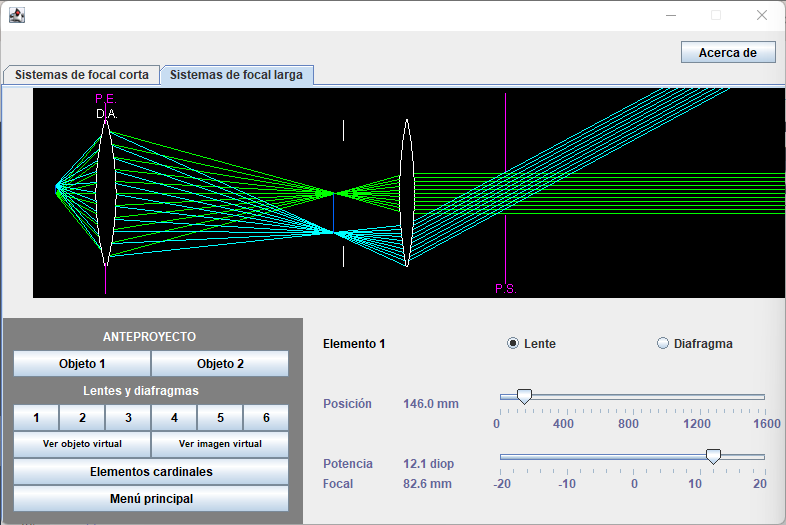
\includegraphics[width=0.51\textwidth]{fotos/parte 2/Microscopio/microscopio_9.png}
    \end{wrapfigure}
    
    \noindent Vamos a preparar un sistema óptico de focal larga con los datos que se nos indica en el informe:
    \begin{itemize}
        \item Lente objetivo de potencia $P = 12.1\ D$ en $146.0\ mm$.
        \item Diafragma
        \item Lente de potencia $P = 6.8\ D$ en $748.0\ mm$.
        \item Objeto real en $s = 45.0\ mm$ con semicampo $2.5^\circ$.
    \end{itemize}

    \clearpage
    \noindent Trabajaremos con este sistema tanto en esta cuestión como en la siguiente. Primero vamos a comentar los elementos cardinales del microscopio tal y como se muestran en la siguiente imagen:
    \\
    \begin{figure}[ht]
        \centering
        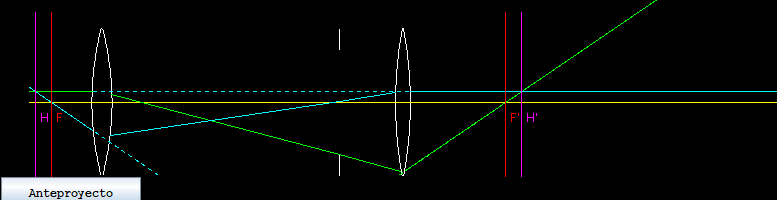
\includegraphics[scale=0.55]{fotos/parte 2/Microscopio/microscopio_9_elementos_cardinales.png}
        \label{fig:microscopio_9_elementos_cardinales}
    \end{figure}
    \\
    
    \noindent En primer lugar, tanto el plano focal imagen como el plano principal imagen se encuentran a la derecha de la segunda lente. De forma análoga, plano focal objeto y plano principal objeto están a la izquierda de la primera lente.
    \\
    
    \noindent Se dice que este sistema es convergente porque el plano focal objeto se encuentra a la derecha del plano principal imagen, es decir, $s_f' > 0$. Además, la imagen que se forma es real puesto que los rayos se cruzan a la izquierda del plano principal imagen.
    \\

    \vspace{0.6cm}
    \textit{\textbf{CUESTIÓN 12.} Observar con la ayuda de un diafragma el tamaño y la orientación de la imagen intermedia.}
    \\
    
    \noindent Para ver el tamaño y orientación de la imagen intermedia, lo que vamos a hacer es situar un diafragma precisamente en la misma posición y ajustar su diámetro de forma que su radio coincida con el tamaño de la imagen. En este caso, lo que queda es lo siguiente:
    \begin{figure}[ht]
        \centering
        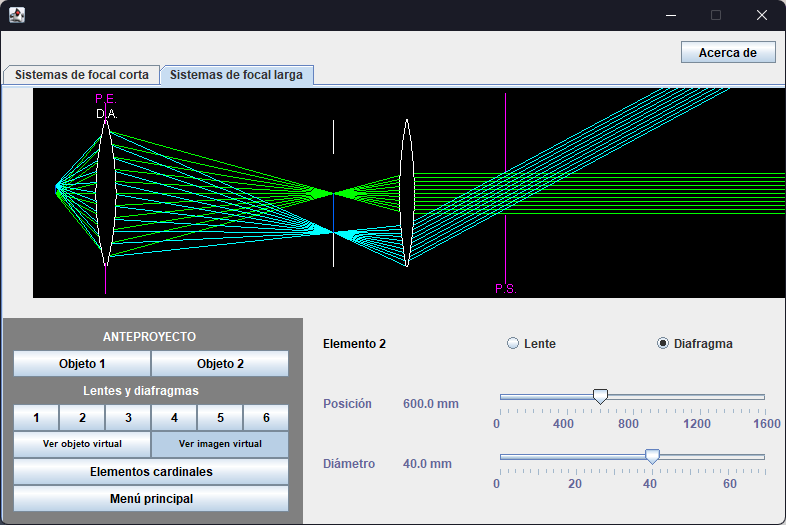
\includegraphics[scale=0.45]{fotos/parte 2/Microscopio/microscopio_10_tamaño_imagen.png}
        \label{fig:microscopio_10_tamañoimagen}
    \end{figure}
    
    \noindent Hemos tenido que fijar el diámetro del diafragma en $\varnothing = 40\ mm$, por lo que podemos afirmar que la imagen intermedia, que además encontramos invertida, tiene un tamaño de $y = \frac12 \varnothing = 20\ mm$.  

    \clearpage
    \subsection{Teleobjetivo}
    \textit{\textbf{CUESTIÓN 13.} Calcula la distancia focal del teleobjetivo propuesto.}
    \\

    \begin{wrapfigure}[7]{l}{0.5\textwidth}
        \vspace{-0.7cm}
        \centering
        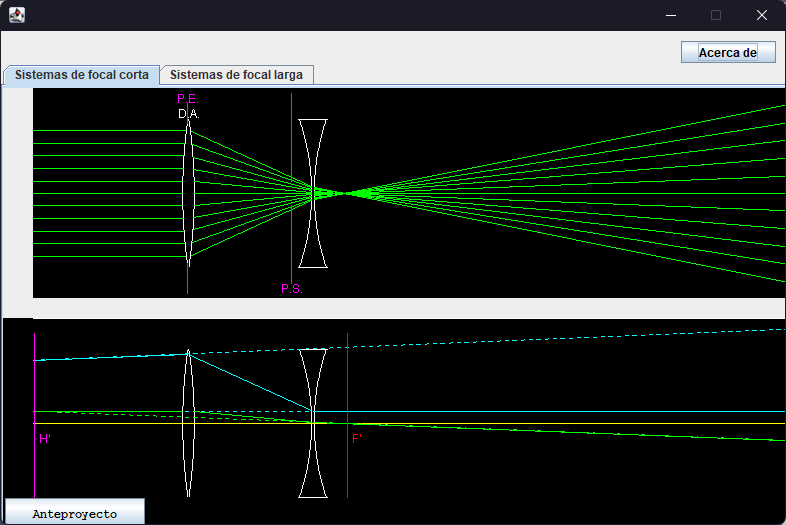
\includegraphics[width=0.48\textwidth]{fotos/parte 2/Teleobjetivo/teleobjetivo_13_elementos_cardinales.png}
    \end{wrapfigure}
    
    \noindent El teleobjetivo que nos proponen tiene las siguientes características:
    \begin{itemize}
        \item Lente convergente con potencia $10\ D$ situada a $111\ mm$.
        \item Lente divergente con potencia $-49.8\ D$ situada a $200\ mm$.
        \item Objeto real en infinito.
    \end{itemize}
    \hspace{0cm}\\
    
    \noindent Para dar la focal total del sistema, tenemos que hacer un pequeño cálculo previo para obtener las focales de ambas lentes, así como la distancia entre ellas.
    \[\begin{cases}
        \begin{aligned}
            &e = 200 - 111 = 89\text{ mm}\\
            &f'_1 = \sfrac{1}{P_1} = \sfrac{1}{10} = 0,1\text{ m} = 100\text{ mm} = -f_1\\
            &f'_2 = \sfrac{1}{P_2} = \sfrac{1}{-49.8} = -0,02\text{ m} = -20\text{ mm} = -f_2
        \end{aligned}
    \end{cases}\]    
    \noindent Ahora aplicamos la ecuación que hemos visto en teoría y sustituimos los valores obtenidos:
    \begin{equation*}
        f' = -\frac{f'_1f'_2}{e-f'_1+f_2} = -\frac{100\cdot (-20)}{89-100+20} = 222.2\ mm
    \end{equation*}
    \\

    \noindent \textit{\textbf{CUESTIÓN 14.} Construye un teleobjetivo invertido utilizando una lente positiva de $15\ D$ y otra negativa de $-50\ D$ (utiliza sistemas de focal corta). Determina su distancia focal. Para estimar las posiciones de H’ y F’, puedes ayudarte de diafragmas.}
    \\

    \begin{wrapfigure}[10]{r}{0.5\textwidth}
        \vspace{-0.7cm}
        \centering
        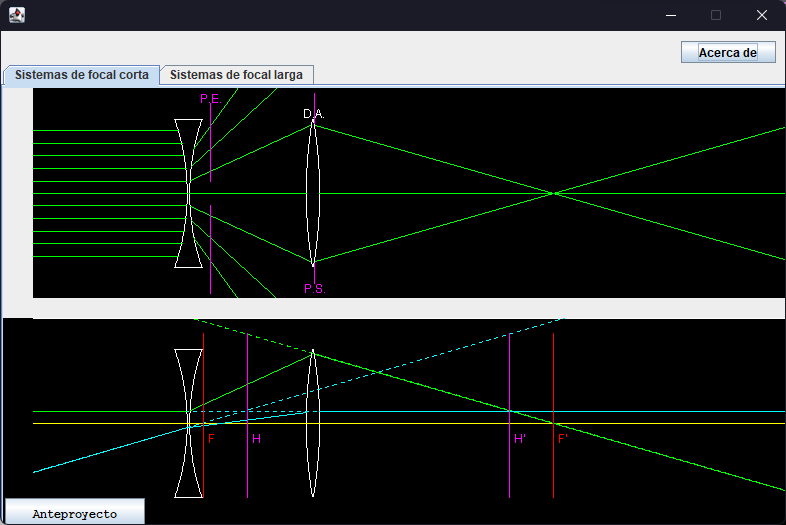
\includegraphics[width=0.48\textwidth]{fotos/parte 2/Teleobjetivo/teleobjetivo_14_invertido.png}
    \end{wrapfigure}
    
    \noindent Nuestro teleobjetivo invertido queda de la siguiente forma:\\

    \noindent Vamos a dar la distancia focal de cada una de las lentes, y por tanto también del sistema, de la misma forma que hemos hecho antes.\\
    
    La diferencia es que ahora tenemos en cuenta que la lente convergente es la segunda:\\ 
    \hspace{0cm}\\
    
    $\begin{cases}
        \begin{aligned}
            &e = 200 - 111 = 89\text{ mm}\\
            &f'_1 = \sfrac{1}{P_1} = \sfrac{1}{-50} = -0,02\text{ m} = -20\text{ mm} = -f_1\\
            &f'_2 = \sfrac{1}{P_2} = \sfrac{1}{15} = 0.067\text{ m} = 67\text{ mm} = -f_2
        \end{aligned}
    \end{cases}
    \Longrightarrow f' = -\frac{f'_1f'_2}{e-f'_1+f_2} = -\frac{100\cdot (-20)}{89-100+20} = 670\ mm$
    \\ 

    \clearpage
    \subsection{Objetivo de focal variable, Zoom}
            \noindent Un objetivo de distancia focal variable es un sistema óptico que puede cambiar el valor de la distancia focal total del sistema modificando la posición de uno o varios elementos ópticos. Vamos a diseñar y representar los objetivos de focal variable que vemos en la tabla. El plano focal imagen F' se sitúa cerca del sensor fotográfico, a $370\ $mm, por lo que utilizaremos un sistema de focal corta.

            \begin{table}[ht]
                \centering
                \begin{tabular}{c|cc|cc|cc}
                    \cline{2-5}
                    \textbf{} &
                      \multicolumn{2}{c|}{\cellcolor[HTML]{010066}{\color[HTML]{FFFFFF} \textbf{Lente 1 (-)}}} &
                      \multicolumn{2}{c|}{\cellcolor[HTML]{010066}{\color[HTML]{FFFFFF} \textbf{Lente 2 (+)}}} &
                      \textbf{} &
                      \textbf{} \\ \hline
                    \rowcolor[HTML]{CBCEFB} 
                    \multicolumn{1}{|c|}{\cellcolor[HTML]{CBCEFB}\textbf{Objeto}} &
                      \textbf{\begin{tabular}[c]{@{}c@{}}Potencia\\ (D)\end{tabular}} &
                      \textbf{\begin{tabular}[c]{@{}c@{}}Posición\\ (mm)\end{tabular}} &
                      \textbf{\begin{tabular}[c]{@{}c@{}}Potencia\\ (D)\end{tabular}} &
                      \textbf{\begin{tabular}[c]{@{}c@{}}Posición\\ (mm)\end{tabular}} &
                      \textbf{\begin{tabular}[c]{@{}c@{}}Separación\\ (mm)\end{tabular}} &
                      \multicolumn{1}{c|}{\cellcolor[HTML]{CBCEFB}\textbf{\begin{tabular}[c]{@{}c@{}}H'F'\\ (mm)\end{tabular}}} \\ \hline
                    \rowcolor[HTML]{DAE8FC} 
                    \multicolumn{1}{|c|}{\cellcolor[HTML]{DAE8FC}Infinito} &
                      -16.6 & 
                       220.7&
                      +20.0 & 
                       242.8&
                       22.1 & 
                       93.15 \\
                    \rowcolor[HTML]{ECF4FF} 
                    \multicolumn{1}{|c|}{\cellcolor[HTML]{ECF4FF}Infinito} &
                      -16.6 & 
                       229.4&
                      +20.0 & 
                       274.5&
                       45.0 & 
                       54.57 \\
                    \rowcolor[HTML]{DAE8FC} 
                    \multicolumn{1}{|c|}{\cellcolor[HTML]{DAE8FC}Infinito} &
                      -16.6 &
                       190.0&
                      +20.0 &
                       300.0&
                       110.0 &
                       25.0 \\ \hline
                \end{tabular}
                \label{table:cuestion15}
            \end{table}

            \textit{\textbf{CUESTIÓN 15.} Representa los diferentes esquemas ópticos comparando los elementos cardinales de dichos sistemas y la posición del plano focal imagen con respecto al resto de elementos. ¿Qué sucede con la cantidad de luz que llega a la imagen final?}            


            \begin{figure}[ht]
                \centering                
                \begin{subfigure}[t]{.49\textwidth}
                    \centering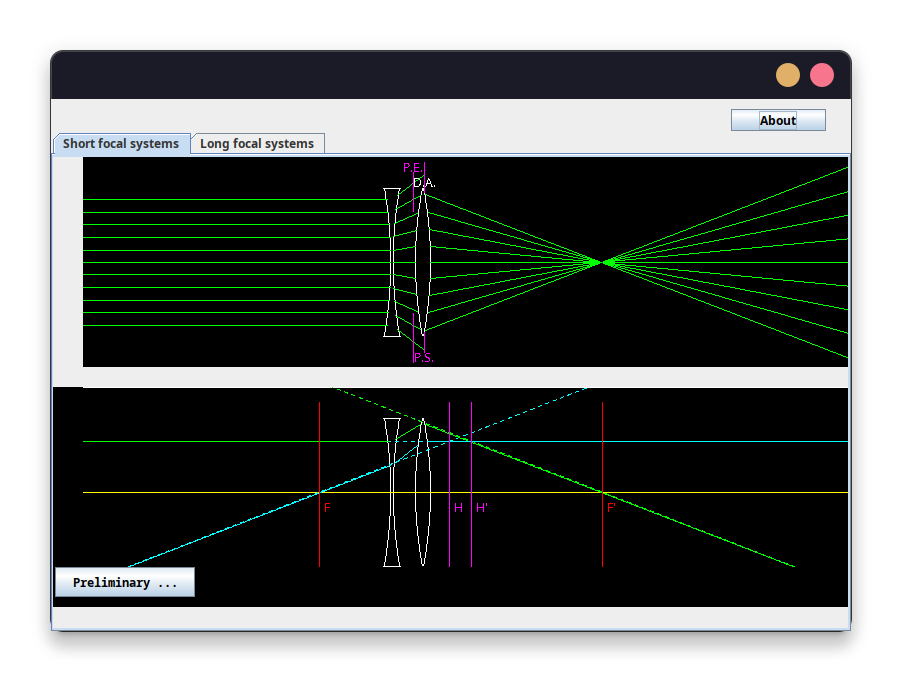
\includegraphics[width=\textwidth]{fotos/parte 2/Zoom/zoom1.png}
                    \caption{Configuración para el Zoom 1}
                \end{subfigure}
                \begin{subfigure}[t]{.49\textwidth}
                    \centering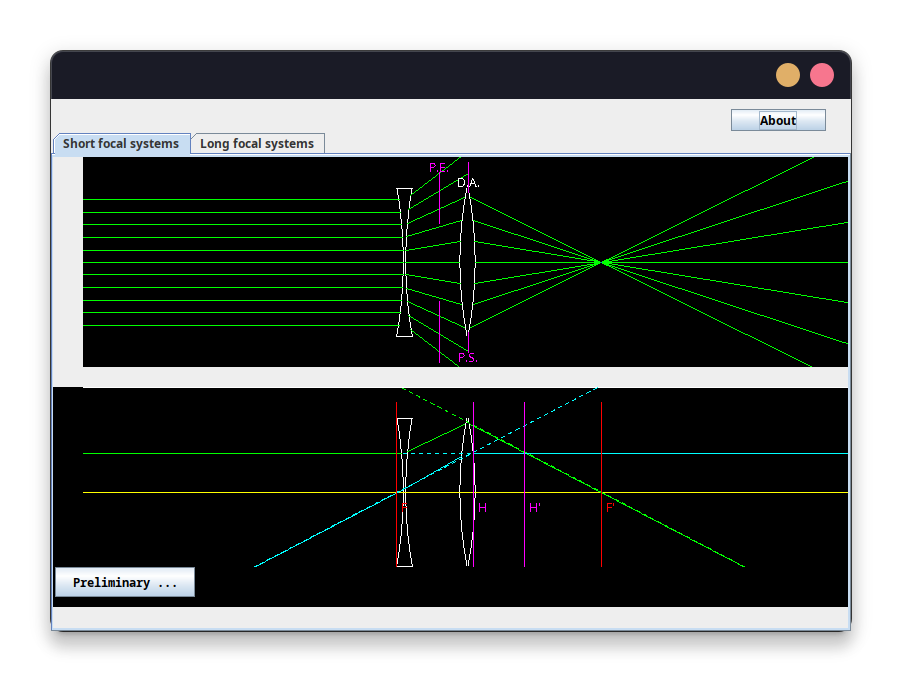
\includegraphics[width=\textwidth]{fotos/parte 2/Zoom/zoom2.png}
                    \caption{Configuración para el Zoom 2}
                \end{subfigure}

                \begin{subfigure}[t]{.49\textwidth}
                    \centering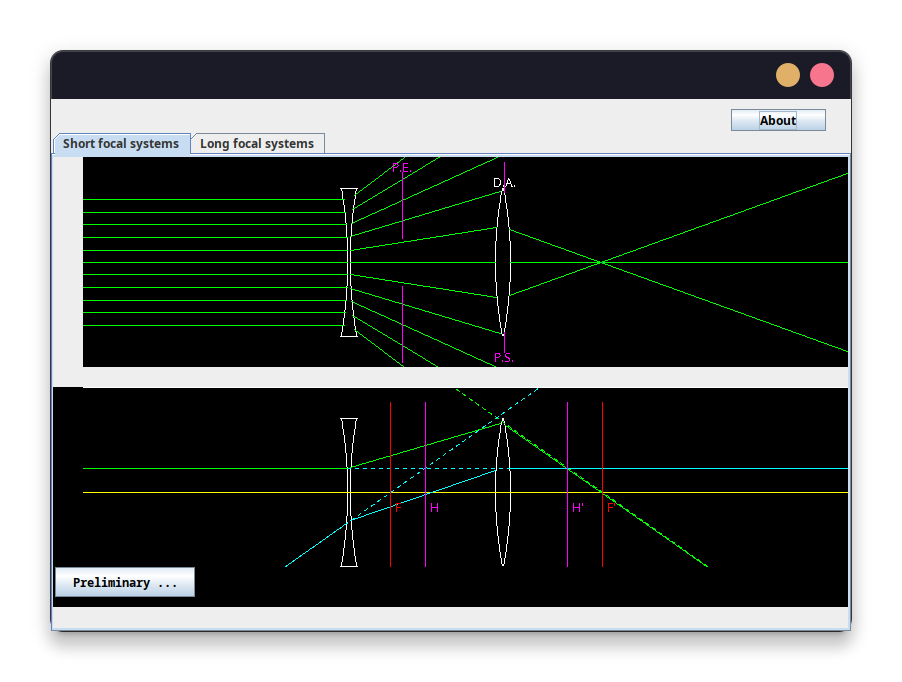
\includegraphics[width=\textwidth]{fotos/parte 2/Zoom/zoom3.png}
                    \caption{Configuración para el Zoom 3}
                \end{subfigure}
            \end{figure}

    \clearpage
    Podemos ver que cuanto menor sea la separación de las lentes, menor será la distancia entre los planos principales. Por el contrario, cuanto menor sea la separación de las lentes, mayor será la distancia entre los planos focales. \\

    A modo de conclusión la separación de las lentes es directamente proporcional con la separación de los planos principales, y inversamente proporcional con la separación de los planos focales.\\

    Observamos como el plano focal imagen se va más a la derecha cuanto menor es la separación de las lentes. La cantidad de luz que llega a la imagen dependerá también de la separación de las lentes, puesto que cuanto más grande es dicha separación, más limita la lente convergente la entrada de luz y por tanto la luz que llega a la imagen será menor.
    
\section{Anexos}
    \subsubsection*{Código de LaTeX que genera este documento:}
        \href{https://www.overleaf.com/read/qgsbffkbrndb#39440e}{OPT1-Práctica1:TrazadoDeRayos.tex}
    \subsubsection*{Código de python que genera las gráficas:}
        \href{https://github.com/vmr48-ua/extras/blob/main/OPT1-P1.py}{OPT1-Práctica1: graficas.py}

\end{document} 